\documentclass[ngerman]{article}

\usepackage{xcolor}
\usepackage{inconsolata}
\usepackage[T1]{fontenc}
\usepackage{pgffor}
\usepackage{graphicx}
\usepackage{fancyhdr}
\usepackage{hyperref}
\usepackage{tcolorbox}
\usepackage[margin=1.2in]{geometry}
\usepackage{biblatex}
\addbibresource{refs.bib}

\hypersetup{
  colorlinks=true,
  linkcolor=blue,
  filecolor=magenta,
  urlcolor=blue,
}

\renewcommand*\familydefault{\ttdefault} %% Only if the base font of the document is to be typewriter style

\newcommand{\topic}[1]{\tcbox[on line,arc=4pt,colframe=white,boxrule=0pt,boxsep=0pt,left=4pt,right=4pt,top=3pt,bottom=2pt,colback=gray!30]{#1}}

% Define a custom command for colored boxes around words
\newcommand{\topics}[1]{%
  \linebreak
  \linebreak
  \foreach \word in {#1} {%
    \topic{\word}%
  }%
  \linebreak
}


\title{WebAssembly-basierte visuelle Programmiersprache \br \small Bachelorarbeit}
\author{Max Richter}

\begin{document}

\pagestyle{fancy}
\fancyhead{} % clear all header fields
\fancyhead[RO,LE]{\textbf{WebAssembly-basierte visuelle Programmiersprache}}
\fancyfoot{} % clear all footer fields
\fancyfoot[LE,RO]{\thepage}
\fancyfoot[LO,CE]{\href{https://github.com/jim-fx/bachelor}{github.com/jim-fx/bachelor}}
\fancyfoot[CO,RE]{Max Richter}

\raggedright

\maketitle
\pagebreak

\tableofcontents

\pagebreak

\section{Einleitung}

\subsection{Hintergrund}
In unserer heutigen digitalisierten Welt spielen Human-Computer Interfaces (HCI's) eine entscheidende Rolle.
Hierbei gibt es eine weite Spanne von Komplexität, von einfach zu bedienenden grafischen Benutzeroberflächen bis zu komplexen Programmiersprachen. 
\br
Visuelle Programmiersprachen (VPL's) bieten hier einen interessanten Mittelweg zwischen diesen beiden Konzepten. Sie bieten programmierunerfahrenen Nutzer/innen die Möglichkeit Programme ähnlich wie in einer textuellen Programmiersprache zu entwickeln.
\br
Es gibt bereits eine Vielzahl von VPL's, die in unterschiedlichen Bereichen Anwendung finden. 
Diese reichen von einfachen Tools wie \textit{Scratch} für Kinder bis zu komplexen Systemen wie \textit{Blender} für 3D-Modellierung und Animation. Vor allem in den Bereichen der prozeduralen Generierung von 3D-Modellen (Blender, Houdini, SpeedTree), Materialien (Blender, Substance-Designer) und Animationen (Blender, Unreal-Engine) finden VPL's Anwendung.
\br
Das Ziel dieser Arbeit ist es eine generalisierte visuelle Programmiersprache zu entwickeln, die leicht erweiterbar und performant ist.
Diese wird als Web-App entwickelt, da dies einen niedrigschwelligen Zugang sowie einen einfachen Verbreitungsweg bietet.
\br
Es gibt bereits einige VPL's die als Web-App konzipiert wurden, so z.B. \href{https://nodered.org}{Node-Red},
\href{https://developers.google.com/blockly}{Blockly} oder \href{https://scratch.mit.edu/}{Scratch}. Diese VPL's benutzen Javascript zur Entwicklung der einzelnen Bausteine und sind sie so relativ einfach zu erweitern da Javascript ohne weitere Kompilierung im Browser ausgeführt werden kann. 
Javascript ist \qt{garbage-collected} und dynamischen typisiert und daher oft nicht die beste Wahl für die Entwicklung von performantem Code im Browser. Diese Merkmale können die Ausführungsgeschwindigkeit beeinträchtigen, da die Garbage-Collection unvorhersehbare Verzögerungen verursachen kann und die dynamische Typisierung zusätzliche Ressourcen zur Laufzeit erfordert, um Typinformationen zu verwalten und Fehler zu vermeiden.
Des Weiteren benötigt Javascript besondere Aufmerksamkeit, um sicherzustellen, das der Code von anderen Nutzer/innen sicher ausgeführt werden kann.
\br
In dieser Bachelorarbeit wird eine VPL entwickelt bei der die einzelnen Bausteine als WebAssembly-Module implementiert sind. 
Dies ermöglicht es neue Bausteine von anderen Entwickler/innen einfach hinzuzufügen und so die Funktionalität der VPL zu erweitern.
Hierbei garantiert WebAssembly eine Plattformunabhängigkeit, hohe Performance und Sicherheit, da der Code in einer virtuellen Maschine ausgeführt wird. \cite{Haas2017}
\br
Außerdem wird die VPL im Kontext einer Web-App entwickelt, die es Nutzer/innen ermöglicht prozedurale 3D-Modelle von Pflanzen zu erstellen. 
Dies bietet eine ausgezeichnete Möglichkeit die Performance der VPL zu testen, da 3D-Modelle oft hohe Datenmengen haben und die Generierung dieser Modelle sehr rechenintensiv sein kann.

\subsection{Problemstellung}

Die Entscheidung die VPL als Web-App zu entwickeln bringt neben den oben genannten Vorteilen auch spezifische Herausforderungen mit sich.
So ist die Sprache in der dynamische Webanwendungen entwickelt werden, Javascript, \qt{garbage-collected} und nicht stark typisiert. 
Dies macht es theoretisch schwieriger performante und robuste Anwendungen zu entwickeln. 
Um die Entwicklung etwas leichter zu gestalten habe ich mich entschieden die VPL in \link[TypeScript]{TypeScript} zu entwickeln, da diese Sprache stark typisiert ist und zu JavaScript kompiliert wird.
\br
Weitere Herausforderungen entstehen durch die Nutzung von WebAssembly. 
WebAssembly führt Code in einer virtuellen Maschine aus, die nicht direkt Zugang auf den Speicher oder Variablen der Host-Umgebung (den Browser) hat.
Innerhalb dieser virtuellen Maschine wird der Code nahe der nativen Geschwindigkeit ausgeführt, was zu einer hohen Performance führt. 
Die Herausforderung besteht darin das die Kommunikation zwischen der Host-Umgebung und dieser virtuellen Maschine relativ langsam ist und so zu einem Engpass führen kann.
\br
Außerdem erlaubt WebAssembly nur sehr wenige numerische Datentypen; 32 und 64 Bit Integer sowie 32 und 64 Bit Floats nach dem IEEE 754 Standard. 
Größere und komplexe Datentypen müssen serialisiert werden, um sie an WebAssembly zu übergeben. 
Um komplexere Werte wieder an die Host-Umgebung zu übergeben, muss diese direkt auf den Speicher der virtuellen Maschine zugreifen.
Zum Glück gibt es Bibliotheken wie \link[WASM-Bindgen]{WASM-Bindgen} die diese Kommunikation abstrahieren und vereinfachen.
\br
Da WebAssembly ein binäres Format ist, wird es selten direkt geschrieben und meistens als Kompilierungsziel für komplexere Programmiersprachen benutzt.
Ich entschied mich für die Programmiersprache \link[Rust]{Rust}, da sie eine starke Typisierung, Performance und Speichersicherheit bietet \cite{bugden2022rust}.
Zusätzlich bietet \link[Rust]{Rust} eine gute Integration mit WebAssembly und ermöglicht es, Rust-Code direkt in WebAssembly zu kompilieren. 
Die \href{https://rustwasm.github.io/}{Rust and WebAssembly domain working group} bietet viele Tools und Bibliotheken an, die die Entwicklung von WebAssembly-Anwendungen in \link[Rust]{Rust} erleichtern.

\subsection{Zielsetzung} 
\label{sec:Zielsetzung}

Das Ziel dieser Bachelorarbeit ist es eine visuelle Programmiersprache zu entwickeln, die \textbf{performant}, \textbf{erweiterbar} und möglichst \textbf{einfach zu bedienen} ist.
Um diese drei Anforderungen laufend zu überprüfen wird die VPL im Kontext einer Web-App entwickelt, die den Nutzer/innen erlaubt prozedurale 3D-Modelle von Pflanzen zu erstellen.
Dieser Anwendungsfall wurde gewählt da die hohen Datenmengen von 3D-Modellen eine gute Möglichkeit bieten die Performance der VPL zu testen.

\subsection{Anforderungen}

\subsubsection{Erweiterbarkeit}

Hiermit ist gemeint, dass das System einfach um neue \link[node_definition]{Node-Definitionen} erweitert werden kann.
\qt{Einfach} heißt in diesem Kontext das ein/e andere/r Programmierer/in möglichst 
schnell in der Lage sein soll eigene WebAssembly-Module zu schreiben welche dann von der VPL geladen und ausgeführt werden können.
Um dies zu erreichen, müssen die Interfaces und Abstraktionen möglichst minimal gehalten werden.
\br
Außerdem sollen die Komponenten, auf die ich in der \link{Architektur} noch genauer eingehen werde, in unterschiedlichen Umgebungen implementiert und ausgeführt werden können.
Vorstellbar wäre zum Beispiel das der/die Nutzer/in den \link[node_graph]{Node-Graph} in einer Web-App bearbeitet, dieser aber in Echtzeit auf einem Server ausgeführt wird. 
Dies erfordert eine möglichst lose Kopplung und die Minimierung des Datentransfers zwischen den einzelnen Komponenten.

\subsubsection{Performance}

Geschwindigkeit von User-Interfaces ist ein wichtiger Indikator für die User-Experience \cite{6876022}. 
Je schneller Nutzende nach einer Änderung das Ergebnis sehen, desto schneller und effizienter können diese iterieren. 

Da diese VPL als Webanwendung entwickelt wird, spielt auch die Ladezeit eine Rolle. 
Hierbei muss darauf geachtet werden diese so kurz wie möglich zu halten.

\subsubsection{User-Experience}

Diese Anforderung ist deutlich schwieriger zu konkretisieren. User-Experience umfasst die gesamte Interaktion von der ersten Interaktion bis zur regelmäßigen Nutzung. In dieser Arbeit wird der Fokus darauf liegen das Erstellen und Bearbeiten von \link[node_graph]{Node-Graphen} so intuitiv und einfach wie möglich zu gestalten.

\subsubsection{Non-Goals}
Die Webplattform bietet viele Möglichkeiten Anwendungen für Nutzer/innen mit Behinderungen angenehmer zu gestalten. 
Die dynamische Struktur einer VPL, sowie spezifische Details der Implementierung machen dies für diese Anwendung ein sehr großes Unterfangen, was im zeitlichen Rahmen dieser Arbeit nicht umsetzbar wäre. So weit wie möglich wird auf Zugänglichkeit geachtet, diese umfassend zu garantieren wird aber nicht Teil dieser Arbeit sein.
\br
Auch die Optimierung für mobile Endgeräte ist nicht vorgesehen, da die Art der Anwendung sich nicht für kleine Bildschirme oder Touch-Interfaces eignet.
\br
Hierbei ist zu erwähnen das diese Ziele nur im Kontext der Bachelorarbeit ausgeklammert werden aber für zukünftige Weiterentwicklung durchaus infrage kommen.

\subsection{Forschungsfragen}
Da die Verwendung von WebAssembly einer der größten Unterscheidungsmerkmal zu anderen VPL's ist, sind die Forschungsfragen spezifisch auf die Eignung von WebAssembly als Grundlage für eine VPL ausgerichtet. Konkret soll dies anhand der folgenden Fragen überprüft werden:
\begin{itemize}
  \item  Inwieweit eignet sich WebAssembly als Grundlage für eine node-basierte visuelle Programmiersprache?  
  \item Welche Auswirkungen haben die spezifischen Vor- und Nachteile von WebAssembly auf die Realisierbarkeit, Funktionalität, Nutzerfreundlichkeit, Performance, Flexibilität und Robustheit einer solchen Programmiersprache?
\end{itemize}

\pagebreak

\subsection{Technologien}

Bei der Wahl der Technologien habe ich versucht Technologien auszuwählen die zukunftssicher sind und den Anforderungen dieser Anwendung entsprechen. Dies bedeutet zum einen das diese Technologien bereits weit verbreitet sind, eine aktive Community haben und aktiv weiterentwickelt werden.

\subsubsection{WebAssembly}
WebAssembly (WASM) ist ein Bytecode-Format für eine Stack-basierte virtuelle Maschine. Es wurde von der WebAssembly Working Group des World Wide Web Consortium (W3C) entwickelt und ist seit 2017 ein offizieller Web-Standard \cite{Haas2017}. 
\br
Es wird hauptsächlich als Kompilierungsziel für kompilierte Programmiersprachen wie C, C++ und \link[Rust]{Rust} benutzt, um diese in Webanwendungen zu integrieren. Im Gegensatz zu Javascript ist WebAssembly nicht \qt{garbage-collected} und ist außerdem stark typisiert.
\br
WebAssembly wurde gewählt, da es erlaubt performanten Code zu schreiben der in allen gängigen Browsern ausgeführt werden kann. 
Zudem kann man durch die Isolation WebAssembly-Module von anderen Entwickler/innen ausführen, ohne das dies ein Sicherheitsrisiko darstellt. Dies macht die Anwendung leicht erweiterbar.
\subsubsection*{WebAssembly Component Model}
Das WebAssembly Component Model ist ein neuer Standard, der es ermöglicht das sich WebAssembly-Module untereinander instanziieren und aufrufen können. \cite{bytecodeallianceIntroductionWebAssembly} 
Dies würde es ermöglichen den \link[runtime_executor]{Runtime-Executor} als WebAssembly-Modul zu implementieren und so die Ausführung der Nodes zu beschleunigen, da der Overhead der Kommunikation zwischen WebAssembly und Javascript vermieden wird. Allerdings gab es erst am 25. Januar 2024 die stabile Veröffentlichung dieses Standards, und zu diesem Zeitpunkt wird er von noch keinem Browser unterstützt.

\subsubsection{WASM-Bindgen \& WASM-Pack}
\label{sec:WASM-Bindgen}

WASM-Bindgen und WASM-Pack sind ein Rust-Bibliotheken, die die Interaktion zwischen Rust und Javascript erleichtern. Sie generieren automatisch die notwendigen Bindings, um Rust- und Javascript-Code miteinander zu verknüpfen. Außerdem helfen sie bei der Kompilierung von Rust-Code in WebAssembly-Module. 
\cite{rustwasmIntroductionwasmbindgen}

\subsubsection{Svelte}
\label{sec:Svelte}

\href{https://svelte.dev/}{Svelte} ist ein deklaratives Frontend-Framework, das sich dadurch auszeichnet auf ein virtuelles DOM zu verzichten und möglichst viel der Arbeit in der Build-Zeit zu erledigen.

\subsubsection{Three.js / Threlte}

Three.js ist der Industriestandard für interaktive 3D-Webanwendung. Es abstrahiert die unterliegende komplexe WebGL-Api und bietet eine Vielzahl von Funktionen und Beispielen. Threlte ist eine Wrapper-Bibliothek um Three.js die es erlaubt Szenen deklarativ zu beschreiben und das Reaktivitätsmodell von Svelte zu nutzen.

\subsubsection{Rust}
\label{sec:Rust}

Rust ist eine von Mozilla entwickelte Programmiersprache, die sich durch ihre Sicherheit und Performance auszeichnet. Sie ist statisch typisiert und besitzt ein Borrow-Checker, der die Speichersicherheit garantiert. \cite{Jung_2020} Rust bietet zum einen die Möglichkeit eng mit dem Speicher zu arbeiten bietet aber auch abstrakte Konzepte wie Traits und generischen Typen und ein mächtiges Makro-System, das mit bei der Entwicklung dieser Anwendung sehr geholfen hat.

\subsubsection{TypeScript}
\label{sec:TypeScript}
TypeScript ist ein Superset von Javascript, das statische Typisierung und andere Features hinzufügt. Es kompiliert zu Javascript und kann daher in allen gängigen Browsers und in der Node.js Laufzeitumgebung ausgeführt werden. Die Sprache wird seit 2012 aktiv von Microsoft entwickelt und hat eine große und aktive Community.

\pagebreak

\section{Theoretischer Rahmen}

\subsection{Definition von visuellen Programmiersprachen}
Eine visuelle Programmiersprache stellt die Komponenten und Verbindungen eines Programms in mehr als einer Dimension dar. Oft ist diese Dimension eine zweidimensionale Fläche auf der die einzelnen Funktionen oder Komponenten eines Systems visuell dargestellt werden. 
Auch wenn textuelle Sprache auf einer zweidimensionalen Oberfläche dargestellt wird, so ist sie meist aus Sicht des Interpreters oder Compilers ein eindimensionaler Stream aus Tokens. \cite{Myers}

\subsection{Klassifikation von visuellen Programmiersprachen}

Nach Burnett\&Mayer können VPL's in 5 verschiedenen Klassen eingeteilt werden \cite{BURNETT1994287}. Diese einzelnen Klassen schließen sich nicht gegenseitig aus und können auch in Kombination verwendet werden.

\subsubsection{\qt{Purely visual languages}}
\qt{Purely visual languages} haben keine textuelle Repräsentation und sind ausschließlich visuell. Ein Beispiel hierfür ist Scratch, das es Nutzern ermöglicht, durch das Zusammensetzen von Blöcken Programme zu erstellen, ohne eine einzige Zeile Code zu schreiben. \cite{mitScratchAbout}

\subsubsection{\qt{Hybrid text and visual Systems}}
\qt{Hybrid text and visual systems} haben eine textuelle Repräsentation, die parallel zur visuellen Repräsentation existiert. 
Ein Beispiel hierfür ist Microsofts \qt{Visual Programming Language}, das Teil von Microsoft Robotics Developer Studio ist und eine hybride Umgebung bietet, in der Nutzer sowohl Code schreiben als auch visuelle Elemente nutzen können. \cite{microsoftIntroduction}

\subsubsection{\qt{Programming-by-example Systems}}
Programming-by-example Systems erlauben es dem Nutzer, ein Programm zu schreiben, indem er die gewünschte Funktionalität in einem Beispiel demonstriert. Etoys, basierend auf Squeak, ist ein Beispiel für ein solches System, bei dem Benutzer durch das Demonstrieren von Aktionen Objekte programmieren können. \cite{squeakSqueakSmalltalk}

\subsubsection{\qt{Constraint-oriented Systems}}
\qt{Constraint-oriented Systems} erlauben es dem Nutzer, Constraints zwischen den Komponenten des Programms zu definieren. SketchPad wäre ein Beispiel für ein solches System, bei dem Benutzer geometrische Formen zeichnen und Constraints zwischen ihnen definieren können. \cite{sutherlandSketchpad}

\subsubsection{\qt{Form-based systems}}
In \qt{Form-based systems} schreiben die Nutzer Programme, indem sie Formulare ausfüllen. 
Ein klassisches Beispiel für ein Formular-basiertes System ist Oracle Forms, 
das eine GUI für Datenbankabfragen und -transaktionen bietet, indem es Benutzern ermöglicht, Formulare auszufüllen, die dann in SQL-Code umgewandelt werden. \cite{wikipediaOracleForms}

\subsection{Historische Vorbilder}

Visuelle Programmiersprachen haben eine lange Geschichte, die bis in die 1960er Jahre zurückreicht. Im folgenden Kapitel werde ich auf einige Meilensteine dieser Geschichte eingehen, welchen Einfluss sie bis heute auf HCI's und VPL's haben und wie sie für diese Arbeit relevant sind.

\subsubsection{SketchPad (1962)}
\label{sec:SketchPad}
\begingroup
\setlength\intextsep{4pt}
\begin{minipage}{\linewidth}
\begin{wrapfigure}{R}{0.5\textwidth}
  \centering
  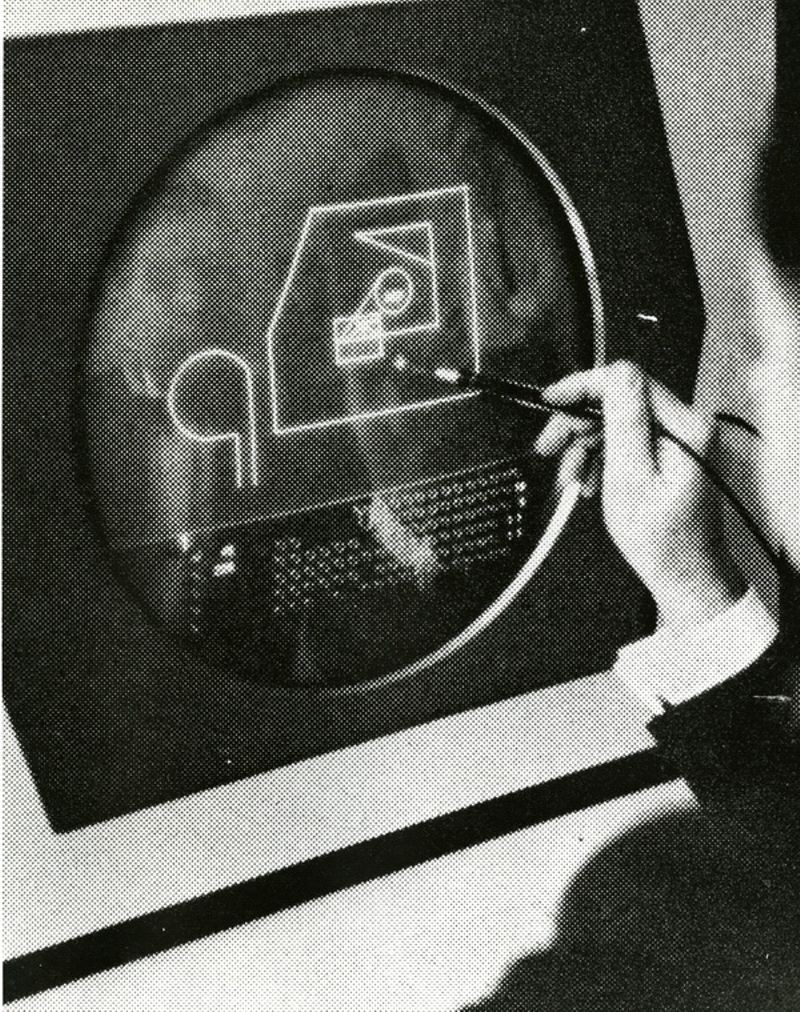
\includegraphics[width=0.4\textwidth]{./graphics/sketchpad-sutherland.jpg} % Change example-image-a with your image filename
  \caption{SketchPad \cite{sutherlandSketchpad}}
\end{wrapfigure}
SketchPad ist ein von Ivan Sutherland entwickeltes Programm das 1963 am MIT veröffentlicht wurde. 
Es benutzte einen Lightpen als Eingabegerät und war das erste Programm, das die Interaktion mit einem Computer über eine grafische Benutzeroberfläche ermöglichte. 
Es erlaubte den Nutzer/innen, geometrische Formen auf einem Bildschirm zu zeichnen und diese zu manipulieren.
  Dabei existierten diese Formen auf einem virtuellen \qt{Papier}, dass der Nutzer bewegen und zoomen konnte. Dieses Konzept von bewegen und Zoomen virtueller Oberflächen war revolutionär für die damalige Zeit.
  Dies wird deutlich durch den Fakt das der Präsentator während der Präsentation von SketchPad \cite{sketchpadDemo} (10:30) keine Worte fand, um diesen Vorgang zu beschreiben. Das Konzept von bewegbaren und zoombaren virtuellen Oberflächen ist heute ein Standard in vielen Anwendungen und wird auch in dieser Arbeit verwendet.
Ein weiteres Feature war die Möglichkeit, Constraints zwischen den Formen zu definieren, ähnlich wie in modernen CAD-Programmen. 
Wenn man sich die Videodemo von SketchPad anschaut fallen viele Paradigmen auf, die wir heute als gegeben ansehen.
Auch wenn SketchPad nicht direkt in die Definition einer VPL passt, war es ein Meilenstein der Entwicklung von grafischen HCI's. Was durch die Verleihung des Turing Awards an Ivan Sutherland 1988 bestätigt wurde.
\end{minipage}
\endgroup

\subsubsection{Pygmalion (1970)}
\begingroup
\setlength\intextsep{2pt}
\begin{minipage}{\linewidth}
\begin{wrapfigure}{L}{0.4\textwidth}
  \centering
  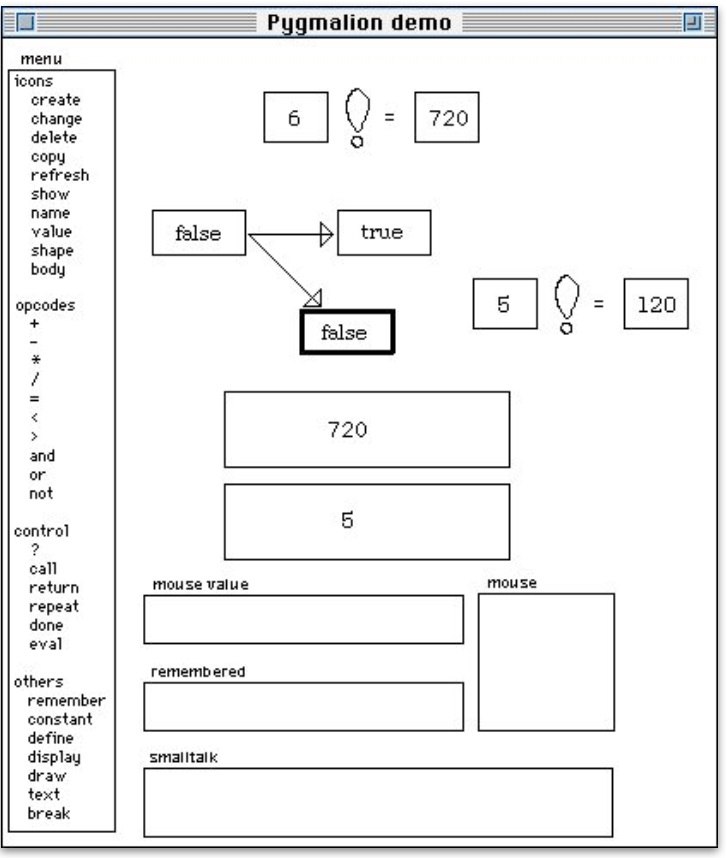
\includegraphics[width=0.4\textwidth]{./graphics/pygmalion.jpg}
  \caption{Fakultät in Pygmalion \cite{smith1975pygmalion}}
  \label{fig:pygmalion_demo}
\end{wrapfigure}

Pygmalion ist eine visuelle Programmiersprache die um 1970 von David Canfield Smith im Rahmen seiner Doktorarbeit entwickelt wurde. Inspiriert wurde sie von der mythischen Figur des Bildhauers Pygmalion der seine Skulpturen zum Leben erwecken konnte.
Die Sprache erlangte nie eine große Verbreitung, war aber ein wichtiger Meilenstein in der Entwicklung von visuellen Programmiersprachen und HCI's.
Pygmalion wurde in Smalltalk implementiert und war eine der ersten visuellen Programmiersprachen. Über eine grafische Oberfläche konnten die Nutzer/innen Blöcke, Icons und Verbindungen erstellen und manipulieren im damit Programme zu definieren.
  Icons waren damals eine Neuerung und wurden von den Entwicklern als \qt{eine Art von visuellen Variablen} bezeichnet. 
  Die Sprache war eine der ersten Beispiele von \qt{Programming By Example} oder PBE. Außerdem war sei eine der ersten Sprachen welche die Verbindung zwischen bestimmten Elementen durch Linien und Pfeile darstellte, was heute ein Standard in vielen VPL's ist.
Die Nutzer/innen konnten Programme schreiben, indem sie die gewünschte Funktionalität in einem Beispiel demonstrieren. 
In Abbildung \ref{fig:pygmalion_demo} wird auf diese Art die Fakultät einer Zahl berechnet. 

\end{minipage}
\endgroup

\subsubsection{Cube (1996)}

\begingroup
\setlength\intextsep{2pt}

\begin{minipage}{\linewidth}
\begin{wrapfigure}{R}{0.4\textwidth}
  \centering
  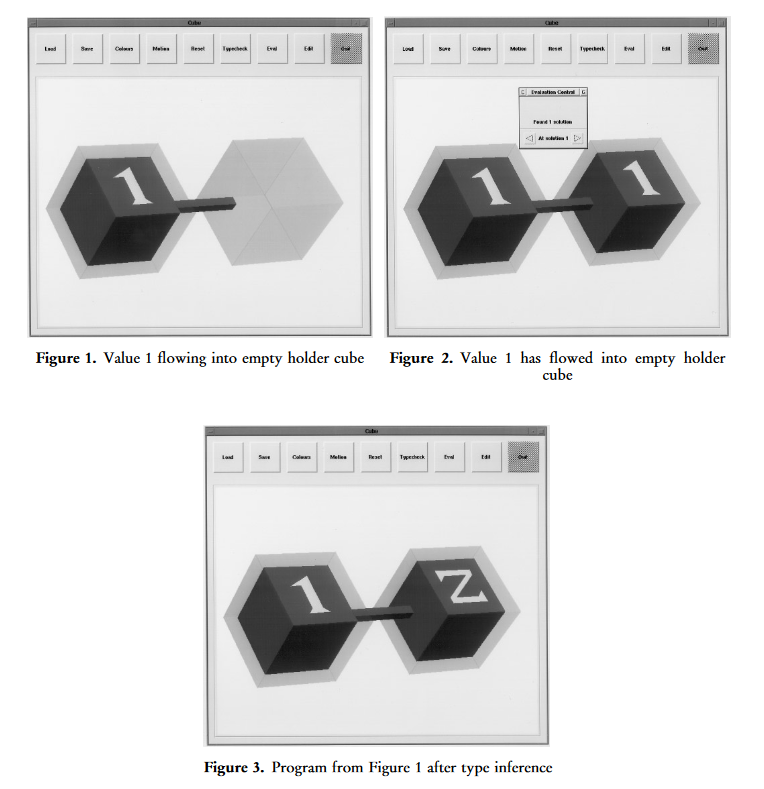
\includegraphics[width=0.4\textwidth]{./graphics/cube_vpl.png} % Change example-image-a with your image filename
  \caption{Datenfluss in Cube \cite{najork1996programming}}
  \label{fig:cube_demo}
\end{wrapfigure}
  \qt{Cube ist eine dreidimensionale, visuelle, statisch typisierte Programmiersprache höherer Ordnung, die für den Einsatz in einer auf virtueller Realität basierenden Programmierumgebung entwickelt wurde.}  \cite{najork1996programming}
In \textit{Cube} werden einzelne Funktionen als, wie der Name schon verrät, Würfel dargestellt. Die Nutzer/innen können dann diese Cubes miteinander verbinden, um Programme zu erstellen.
Canfield geht in seiner Arbeit spezifisch auf den Vergleich zu Rohren und Wasserfluss ein. Somit bedient sich \textit{Cube} einer für Menschen relativ intuitiven Darstellung von Wasserfluss durch Rohre, um den Datenfluss innerhalb des Programms darzustellen.
  Ein interessantes Detail hierbei ist, das diese \qt{Rohre} keine Richtung haben und Daten in beide Richtungen fließen können. 
Da \textit{Cube} eine höhere Programmiersprache ist, können die Cubes auch als Argumente an andere Cubes übergeben werden. Dies ermöglicht es, komplexe Programme zu erstellen, die aus vielen einzelnen Cubes bestehen. 
\br
Dieses Konzept ist relevant für meine persönliche Arbeit, siehe \link[parameter_nodes]{parametrisierte Nodes}.

\end{minipage}
\endgroup
\pagebreak

\subsection{Node-basierte visuelle Programmiersprachen}
In meiner Recherche nach modernen VPL's habe ich mich spezifisch auf node-basierte VPL's konzentriert die entweder durch ihre Popularität oder ihre Spezifizierung relevant für diese Arbeit sind.

\subsubsection{Node-RED}

Node-RED ist eine webbasierte Programmier- und Ausführungsumgebung die auf Nodes basiert und es den Nutzern ermöglicht, diese Nodes miteinander zu verknüpfen, um \qt{Flows} zu erstellen. 
Es wurde 2013 von IBM entwickelt und ist seit 2016 teil der OpenJS Foundation (damals JS Foundation).
\cite{nodered}

\begin{figure}[htbp]
  \centering
  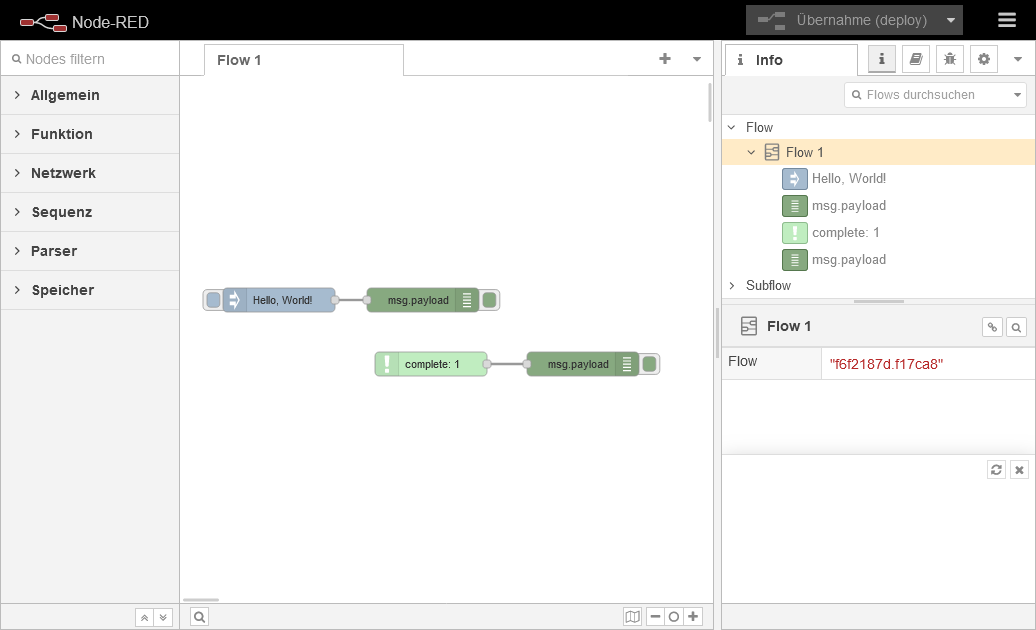
\includegraphics[width=0.7\textwidth]{./graphics/node-red-3_1_8.png}
  \caption{Screenshot Node Red v3.1.8}
  \label{fig:node_red}
\end{figure}

Node-RED findet vor allem Anwendung in den Bereichen IoT und Home Automation, da es eine Vielzahl von Anbindungen an verschiedene Geräte und Dienste bietet. 
Node-RED ist ein Beispiel für sogenanntes datenstromorientierte Programmierung, bei dem die Daten durch die Nodes fließen und diese verarbeiten. Das heißt es gibt keine einmalige Ausführung, sondern das System kann kontinuierlich Daten verarbeiten und auf externe Events reagieren. Im Gegensatz zu der in dieser Arbeit entwickelten VPL ist Node-Red nicht auf WebAssembly basiert und ist nicht generalisiert.


\pagebreak
\subsubsection{Blender}
Blender ist eine weitverbreitete open-source 3D Modellierungs- und Animationssoftware. Blender bietet node-basierte Interfaces zur Erstellung von Materialien, Texturen und Geometrien an. 
\cite{blender}
Für diese Arbeit ist Blender relevant, da es sich auch mit dem Erstellen von 3D-Modellen beschäftigt.

\begin{figure}[htbp]
  \centering
  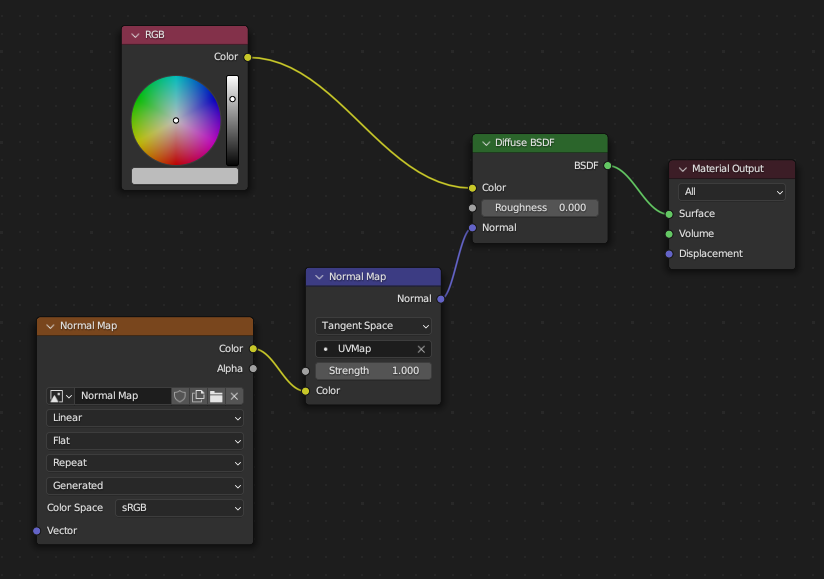
\includegraphics[width=0.6\textwidth]{./graphics/blender-shader.png}
  \caption{Screenshot Blender 3.5 Shader Editor}
  \label{fig:blender-shader}
\end{figure}

Vor allem die User-Experience der Blender Node-Editoren ist ein großer Vorteil. So bietet Blender für die meisten oft benötigten Funktionen Shortcuts an, die es ermöglichen, schnell und effizient zu arbeiten.
Ähnlich wie in Node-RED ist der Datenfluss der westlichen Leserichtung angepasst, von links nach rechts. Dies ermöglicht es, den Datenfluss intuitiv zu verfolgen und zu verstehen.
\br
Im Gegensatz zum Shader Editor (sieht Abbildung \ref{fig:blender-shader}) bietet der Geometry Node Editor die Möglichkeit komplexere Setups zu erstellen. So gibt es zum Beispiel \qt{Repeat Zones}  die es ermöglichen eine Gruppe von Nodes arbiträr oft zu wiederholen.
\br
Außerdem bietet Blender umfassende Tastaturkürzel an die es erlaubt sehr schnell und effizient zu arbeiten. Auch in dieser Arbeit soll darauf geachtet werden, dass die Nutzer/innen möglichst effizient arbeiten können.

\begin{figure}[htbp]
  \centering
  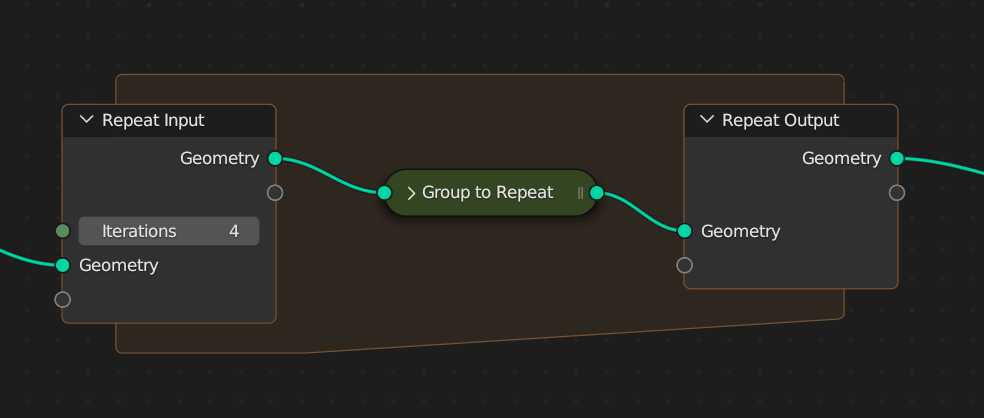
\includegraphics[width=0.6\textwidth]{./graphics/modeling_geometry-nodes_repeat_zone.png}
  \caption{Blender 4.1 Repeat Zone \cite{blenderRepeatZone}}
  \label{fig:blender-repeat}
\end{figure}

\pagebreak

\subsubsection{SpeedTree}

\begin{figure}[htbp]
  \centering
  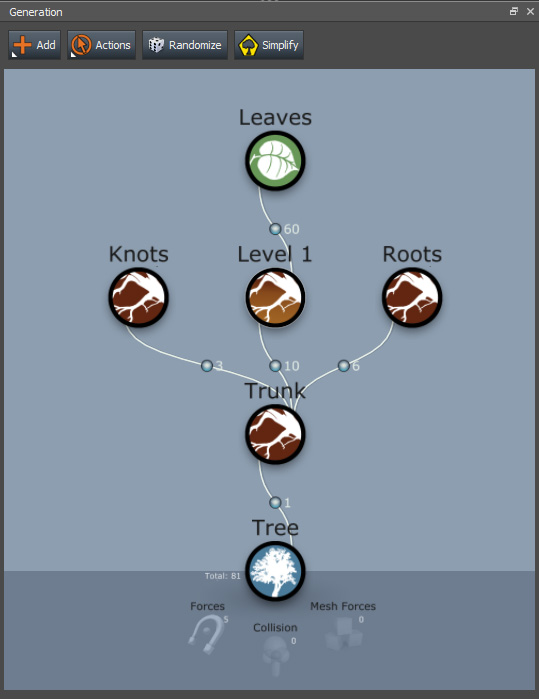
\includegraphics[width=0.6\textwidth]{./graphics/generationeditor_7_speedtree.jpg}
  \caption{SpeedTree Screenshot \cite{speedtreeGettingstartedSpeedTree}}
  \label{fig:blender-repeat}
\end{figure}

SpeedTree ist eine Software zur Erstellung von 3D-Modellen von Pflanzen. Der Nutzer legt über ein node-basiertes Interface die unterschiedlichen Teile eine Pflanze fest und kann so sehr detaillierte und realistische Modelle erstellen. SpeedTree wird seit 2000 von Interactive Data Visualization Inc. entwickelt und findet vor allem Anwendung in der Spieleindustrie. \cite{speedtreeGettingstartedSpeedTree}.
\br
Im Gegensatz zu Blender und Node-RED ist SpeedTree ein sehr spezialisiertes Tool. Außerdem ist es nicht open-source und nicht kostenlos. Auch gibt es keine Möglichkeit, eigene Nodes zu erstellen oder die Software zu erweitern.

\pagebreak

\section{Konzept}

Die in dieser Arbeit entwickelte VPL nutzt einen node-basierten Ansatz. 
\link[node]{Nodes} sind in diesem Kontext einzelne Bausteine die ähnlich wie eine Funktion in einer textuellen Programmiersprache funktionieren.
Das heißt, sie nehmen Argumente entgegen, verarbeiten diese und geben ein Ergebnis zurück.
\br
Die einzelnen Argumente können entweder direkt über das Interface einer \link[node]{Node} definiert werden oder in dem der/die Nutzer/in das Ergebnis einer anderen \link[node]{Node} mit diesem Argument verknüpft.
Bei der visuellen Gestaltung lehnt sich die VPL sehr an die verschiedenen Node-Editoren in Blender an.
\br
Die einzelnen \link[node]{Nodes} sind hierbei jeweils Instanzen eines WebAssembly-Moduls. 
Dies erlaubt es das System um neue Node-Definitionen zu erweitern, indem man eine einzelne WebAssembly Dateien lädt.
Woher diese Dateien kommen ist dabei egal, sie können von der Festplatte, einem Server oder aus dem lokalen Speicher geladen werden.
\br
Die Verbindungen mehrerer \link[node]{Nodes} stellt einen \link[node_graph]{Node-Graph} dar. 
Dieser \link[node_graph]{Node-Graph} kann als JSON-Objekt serialisiert und deserialisiert werden und so gespeichert und geladen werden.
\br
In Abbildung \ref{sec:PURE_GRAPH} ist ein Beispiel für einen \link[node_graph]{Node-Graph} dargestellt. 
Der Datenfluss ist von links nach rechts und die Verbindungen zwischen den Nodes sind gerichtet.


\begin{figure}[htbp]
    \centering
    \begin{minipage}[b]{0.8\textwidth}
        \centering
        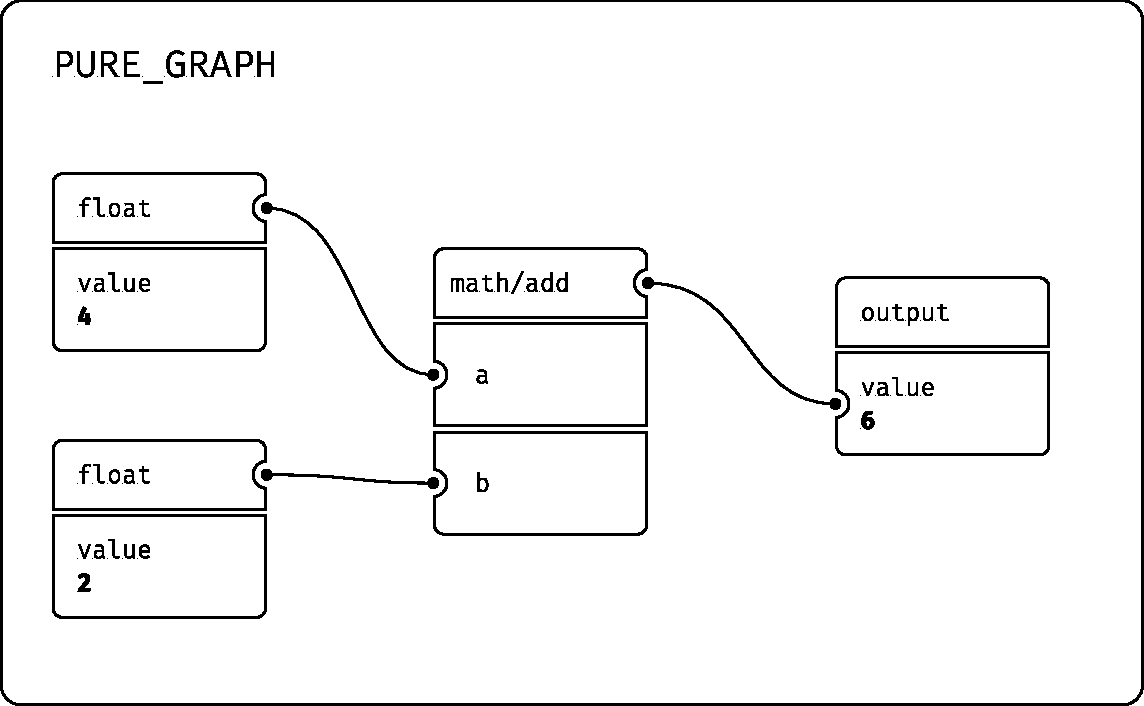
\includegraphics[width=\textwidth]{graphics/PURE_GRAPH.pdf}
        \caption{Darstellung eines \link[node_graph]{Node-Graph}}
        \label{sec:PURE_GRAPH}
    \end{minipage}
\end{figure}

\pagebreak


\subsection{Architektur}
\label{sec:Architektur}
Die VPL muss bestimmte funktionale Anforderungen erfüllen um nutzbar zu sein:
\begin{itemize}
  \item Die Nutzer/innen müssen mit ihr interagieren können.
  \item Die VPL muss dynamisch neue Nodes laden können.
  \item Während die Nutzer/innen mit der VPL interagieren, müssen die Nodes ausgeführt werden.
\end{itemize}
Aus den Anforderungen und dem Konzept ergibt sich folgende dreiteilige Architektur:
\br
Das \link[node_interface]{Node-Interface} ist für das visuelle Interface zuständig, hier interagieren Nutzer/innen mit dem \link[node_graph]{Node-Graph}.
\br
Der \link[runtime_executor]{Runtime-Executor} ist für die Ausführung der Nodes zuständig. Er nimmt einen serialisierten \link[node_graph]{Node-Graph} entgegen und gibt das Ergebnis zurück.
\br
Die \link[node_registry]{Node-Registry} ist für das Verwalten der \link[node_definition]{Node-Definitionen} zuständig. Die beiden anderen Komponenten laden aus ihr die einzelnen WebAssembly-Binärdateien der Nodes.
\br
In Abbildung \ref{fig:overview_sequence} ist in einem Sequenzdiagramm dargestellt wie die drei Komponenten zusammenarbeiten.

\begin{figure}[hbtp]
    \centering
    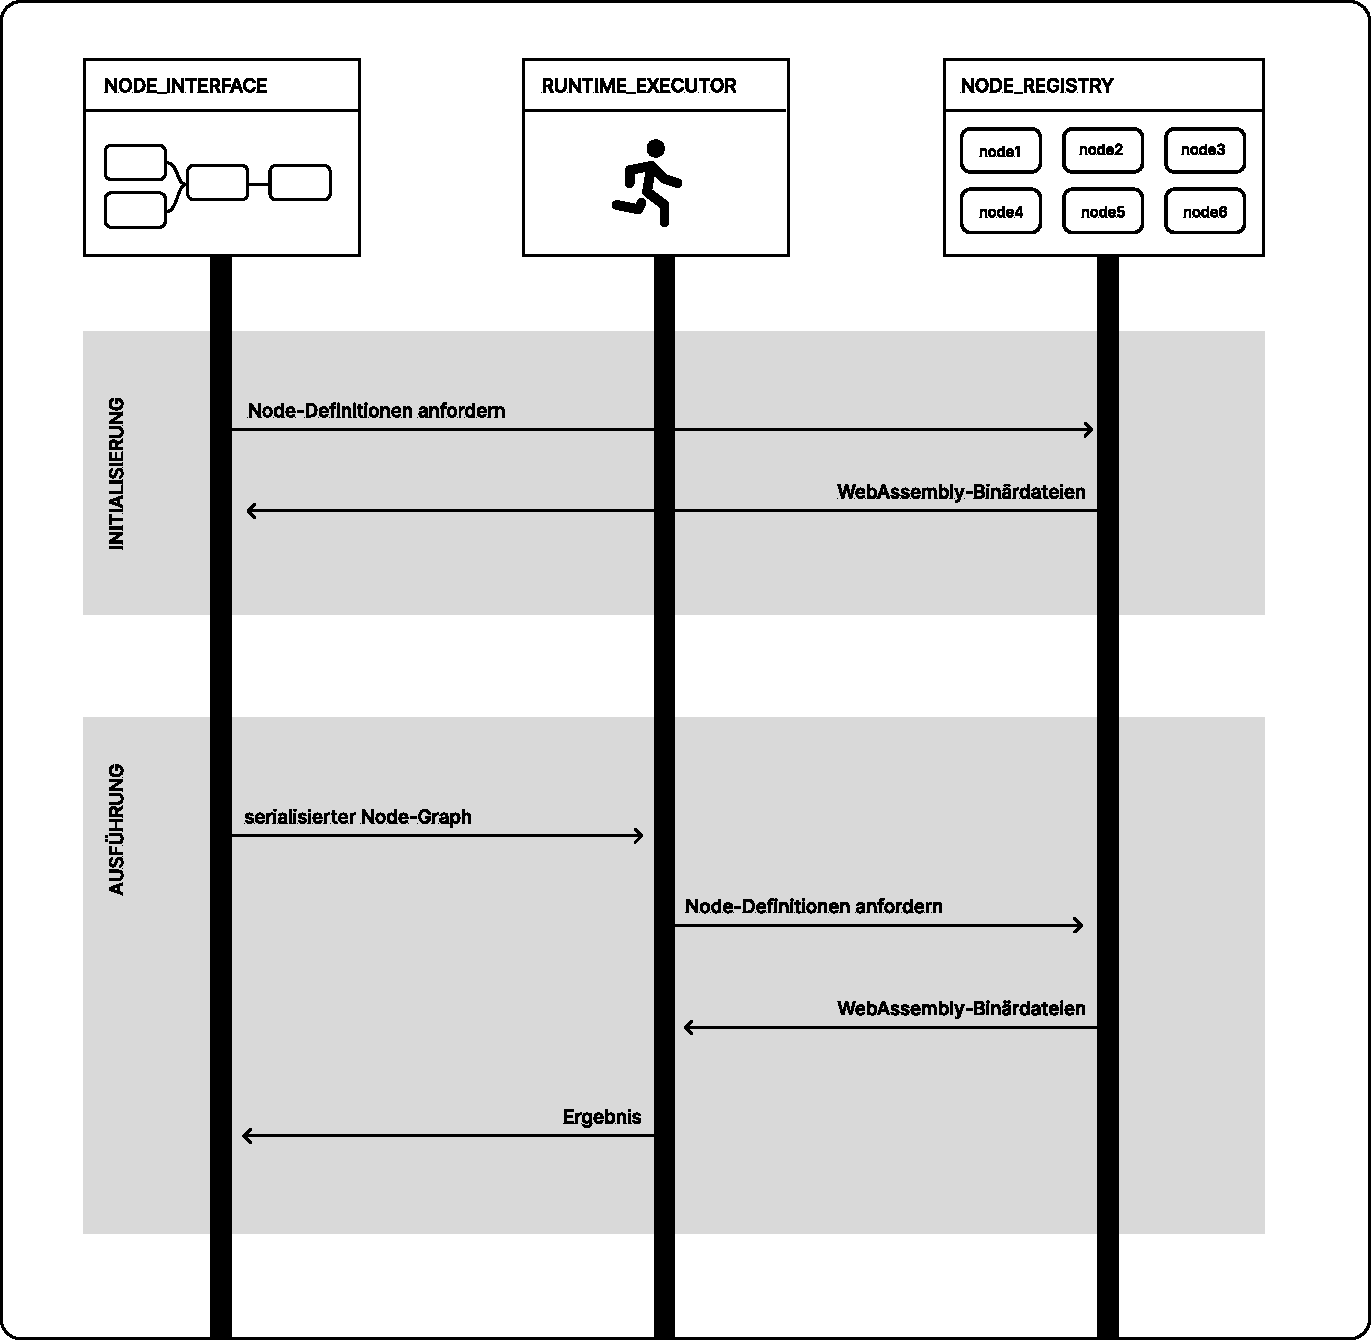
\includegraphics[width=1\textwidth]{graphics/OVERVIEW_SEQUENCE.pdf}
    \caption{Sequenzdiagramm der Architektur}
    \label{fig:overview_sequence}
\end{figure}

\pagebreak

\subsubsection{Datentypen}

Die Datentypen wurden möglichst minimal gehalten. Dies dient zum einen dem Ziel das gesamte System so einfach und verständlich wie möglich zu halten, und zum
anderen macht es die Serialisierung und Deserialisierung der Daten schneller.
\br
Die drei Hauptdatentypen sind  \link[data_node_type]{Node-Definition}, \hyperref[fig:data_node]{Node},  und \hyperref[fig:data_node_graph]{Node-Graph}. 

\subsubsection*{Node-Definition}

\begin{figure}[htbp]
  \begin{code}
    \begin{minted}{typescript}
type NodeDefinition = {
  id: string;
  inputs?: Record<string, NodeInput>
  outputs?: string[];
  execute?: (args: Int32Array) => Int32Array;
}

// Beispiel einer Math Node
const mathNodeType: NodeDefinition = {
  id: "max/plantarium/math",
  inputs: { 
    op_type: { type:"select", options: ["add","subtract","multiply","divide"] }, 
    a: { type: "float" }, 
    b: { type: "float" } 
  },
  outputs: ["float"],
  execute: (inputs) => {
    // Implementierung der Math Node
  }
}
    \end{minted}
  \end{code}

  \caption{Datenstruktur der \link[node_definition]{Node-Definition} (TypeScript)}
  \label{sec:data_node_type}

\end{figure}

Die Node-Definition besteht aus einer \topic{id}, \topic{inputs}, \topic{outputs} und einer \topic{execute} Funktion. Die \topic{inputs} einer \link[node]{Node} können unterschiedliche \topic{type} Werte haben, beispielsweise:

\begin{itemize}
  \setlength\itemsep{0.0em}
  \item float
  \item integer
  \item boolean
  \item select
  \item vec3
\end{itemize}

Über diese \topic{inputs} wird festgelegt welche Argumente eine \link[node]{Node} entgegennimmt.
Im \link[node_interface]{Node-Interface} werden diese dann als Eingabefelder dargestellt. Außerdem legen diese Inputs fest welche \link[node]{Nodes} mit dieser \link[node]{Node} verbunden werden können. 
\br
Ein weiteres Attribut eines \topic{inputs} ist \topic{setting}. So können die Nutzer Argumente festlegen die global für den ganzen \link[node_graph]{Node-Graph} gelten und nicht direkt von einer \link[node]{Node} abhängen. Ein Beispiel aus der Entwicklung wäre hier die \topic{resolution}. Diese legt fest wie viele Vertices eine \link[node]{Node} für ein 3D-Modell generieren soll. Das \link[node_interface]{Node-Interface} konstruiert aus allen \topic{settings} ein globales Einstellungsmenü.
\br
Außerdem gibt es bestimmte Input-Typen die besondere Funktionen haben. So kann eine \link[node]{Node} zum Beispiel einen Input mit \topic{\{"type":\\"\\seed"\}} festlegen, und diesem wird bei der Ausführung durch den \link[runtime_executor]{Runtime-Executor} ein zufälliger Wert zugewiesen.
\br
Einige andere Attribute wurden ausgeklammert um die Lesbarkeit zu erhöhen. So kann ein \topic{input} noch ein \topic{label}, ein \topic{default} und eine \topic{description} haben.

\subsubsection*{Node}

\begin{figure}[htbp]
  \begin{code}
    \begin{minted}{typescript}
type Node = {
  id: number;                       // Primäre ID der Node
  type: string;                     // Type der Node, bsp: max/plantarium/math
  props?: Record<string, any>,      // Daten der Node
  position: [x: number, y: number]  // Visuelle Position
}

const exampleNode: Node = {
  id: 5,
  type: "max/plantarium/math",
  props: { op_type: 0, a: 400, b: 20},
  position: [60, 90]
}

    \end{minted}
  \end{code}

  \caption{Datenstruktur einer \link[node]{Node} (TypeScript)}
  \label{fig:data_node}

\end{figure}

Eine \link[node]{Node} ist eine Instanz einer \link[node_definition]{Node-Definition}. Die Datenstruktur besteht aus einer \topic{id}, einem \topic{type}, optionalen \topic{props} und einer \topic{position}. 
Dieser Datentype findet vorallem Anwendung im \link[node_interface]{Node-Interface}, während der Laufzeit und der Serialisierung und Deserialisierung.
\br
Die \topic{id} ist inkrementell und dient zur eindeutigen Identifikation der Node. Der \topic{type} verbindet eine \link[node]{Node} mit einer \link[node_definition]{Node-Definition}.
Die \topic{props} sind die Argumente die an die \topic{execute} Funktion der \link[node_definition]{Node-Definition} übergeben werden.

\subsubsection*{Node-Graph}

\begin{figure}[htbp]
  \begin{code}
    \begin{minted}{typescript}
type NodeGraph = {
  id: number;                                 // Primäre ID des Graphen
  nodes: Node[];                              // Liste aller Nodes
  edges: [number, number, string][];  // Liste aller Verbindungen
}
    \end{minted}
  \end{code}

  \caption{Datenstruktur eines \link[node_graph]{Node-Graph} (TypeScript)}
  \label{fig:data_node_graph}

\end{figure}

Der \link[node_graph]{Node-Graph} besteht aus einer \topic{id}, einer Liste aller \link[node]{Nodes} und einer Liste aller Verbindungen. 
Die Verbindungen sind jeweils ein Tupel aus der \topic{id} der \link[node]{Node} von der die Verbindung ausgeht, der \topic{id} der \link[node]{Node} zu der die Verbindung geht, und der \topic{id} des \topic{inputs} der empfangenden Node.

\pagebreak

\subsubsection{Node-Interface}
Abbildung \ref{fig:overview_sequence}
\label{sec:node_interface}
\cmt{Visuelles Interface für den Node-Graph}

\subsubsection{Node-Registry}
\label{sec:node_registry}

Die \link[node_registry]{Node-Registry} ist für das Verwalten der \link[node_definition]{Node-Definitionen} zuständig. Konzeptuell funktioniert sie ähnlich wie die Package-Manager der gängigen Programmiersprachen, z.B. \href{https://www.npmjs.com/}{npm} oder \href{https://crates.io/}{crates.io}.
\br
Damit diese \link[node_registry]{Node-Registry} erweiterbar ist wurde ein eigenes ID-Schema für die \link[node_definition]{Node-Definitionen} entworfen. Dies besteht aus einer \topic{user-id} einem \topic{namespace} und der \topic{node-id}. 
Ein Beispiel aus der Entwicklung wäre \topic{max/plantarium/branch}.
\br
Die \topic{user-id} ist die ID des/der Entwicklers/Entwicklerin und dient dazu, die Nodes zu gruppieren. Der Namespace gruppiert Nodes die zusammen funktionieren. So kann das System der \link[HON]{Higher-Order Nodes} nur für Nodes in dem \topic{plantarium} Namespace implementiert werden und andere Namespaces können andere Implementierungen haben.
\br
Die \topic{node-id} muss individuell innerhalb eines \topic{namespace} sein. 
\subsubsection*{Non-Goals}
Obwohl im Design darauf geachtet wurde die \link[node_registry]{Node-Registry} so erweiterbar wie möglich zu machen, wurde darauf verzichtet Funktionen die eine \qt{echte} Registry haben sollte zu implementieren. So gibt es keine Ansätze zur Versionierung, auch auf Authentifizierung und Autorisierung wurde verzichtet.

\subsubsection{Runtime-Executor}
\label{sec:runtime_executor}

Der \link[runtime_executor]{Runtime-Executor} ist für die Ausführung eines \link[node_graph]{Node-Graphen} zuständig.

\pagebreak

\subsubsection{Parametrisierte Nodes}
\label{sec:parameter_nodes}
In vorherigen Abschnitten wurde der Vergleich zwischen \link[node]{Nodes} und Funktionen gezogen. Dies hat den Vorteil, dass es das Konzept etwas leichter verständlich macht.
Es gibt jedoch Situationen, in denen es sinnvoll ist, von dem Konzept einer Node als reiner Funktion abzuweichen, damit die VPL zum einen flexibler und zum anderen einfacher zu bedienen ist. Hier werde ich nun zwei Beispiele für solche Situationen vorstellen.
\subsubsection*{Random Problem}
In Abbildung \ref{fig:random_problem} ist ein beispielhafter Aufbau eines \link[node_graph]{Node-Graphen} dargestellt. Wären die \topic{random} Nodes als reine Funktion implementiert würde sie nur einmal ausgeführt und die beiden \topic{math/add} Nodes würden das gleiche Ergebnis produzieren. Dies wäre für die meisten Nutzenden ein überaschendes Ergebnis.
\br
Eine mögliche Lösung wäre, die \topic{random} Node für jede ihrer ausgehenden Verbindungen separat auszuführen. 
Dies könnte jedoch zur unnötigen Mehrfachausführung von Nodes führen, die dies nicht erfordern.
Außerdem erschwert dies das Caching von Node-Ergebnissen, da nicht nur die Node-Parameter, sondern auch die Anzahl der ausgehenden Verbindungen das Ergebnis beeinflussen würden.
\br
Ein weiterer Nachteil ist das für dieses Konzept die Ausführung der Nodes nicht mehr nur in eine Richtung verläuft. Das könnte zu konzeptioneller Verwirrung und Komplexität führen.
\br
\begin{figure}[htbp]
  \centering
  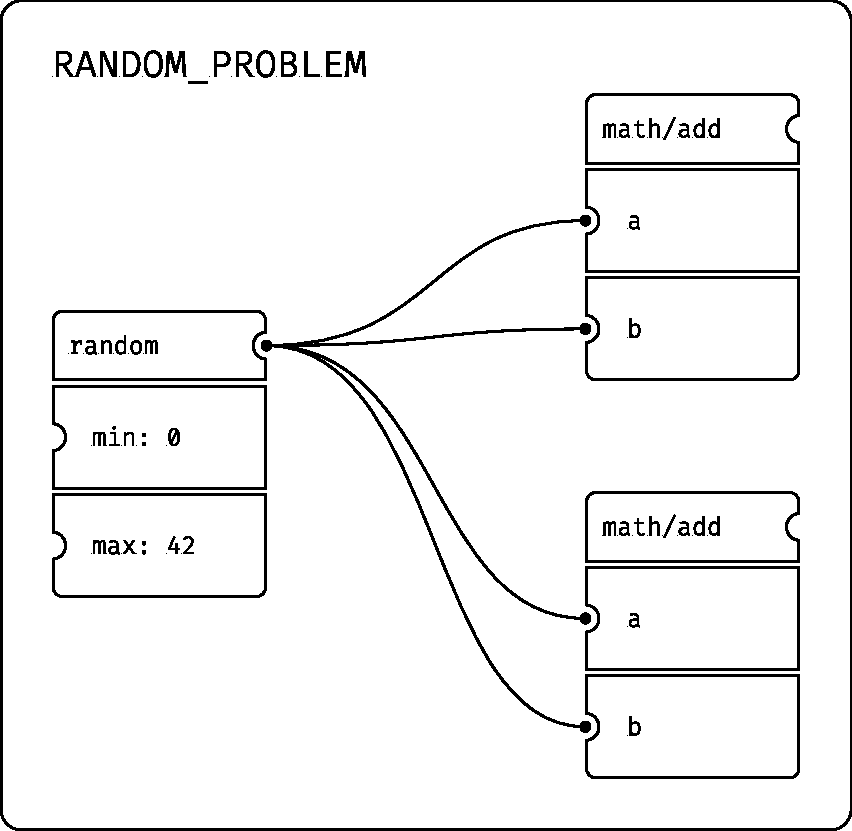
\includegraphics[width=0.5\textwidth]{graphics/RANDOM_PROBLEM.pdf}
  \caption{Illustration eines Problems mit der \texttt{random} Node}
  \label{fig:random_problem}
\end{figure}

\pagebreak

\subsubsection*{Noise Problem}

Ein weiteres Problem soll durch Abbildung \ref{fig:noise_problem} verdeutlicht werden. 
Die hypothetische \topic{cylinder} Node generiert 3D-Modelle von Zylindern. Sie hat einen Input für den Radius, die Höhe und die Anzahl der generierten Zylinder. 
\br
Wenn die vorherigen Nodes als pure Funktionen modelliert wären, würde diese Node Ergebnis A produzieren, da die \topic{noise} Node nur einmal ausgeführt wird. Die meisten Nutzenden würden jedoch eher Ergebnis B erwarten.

\begin{figure}[htbp]
  \centering
  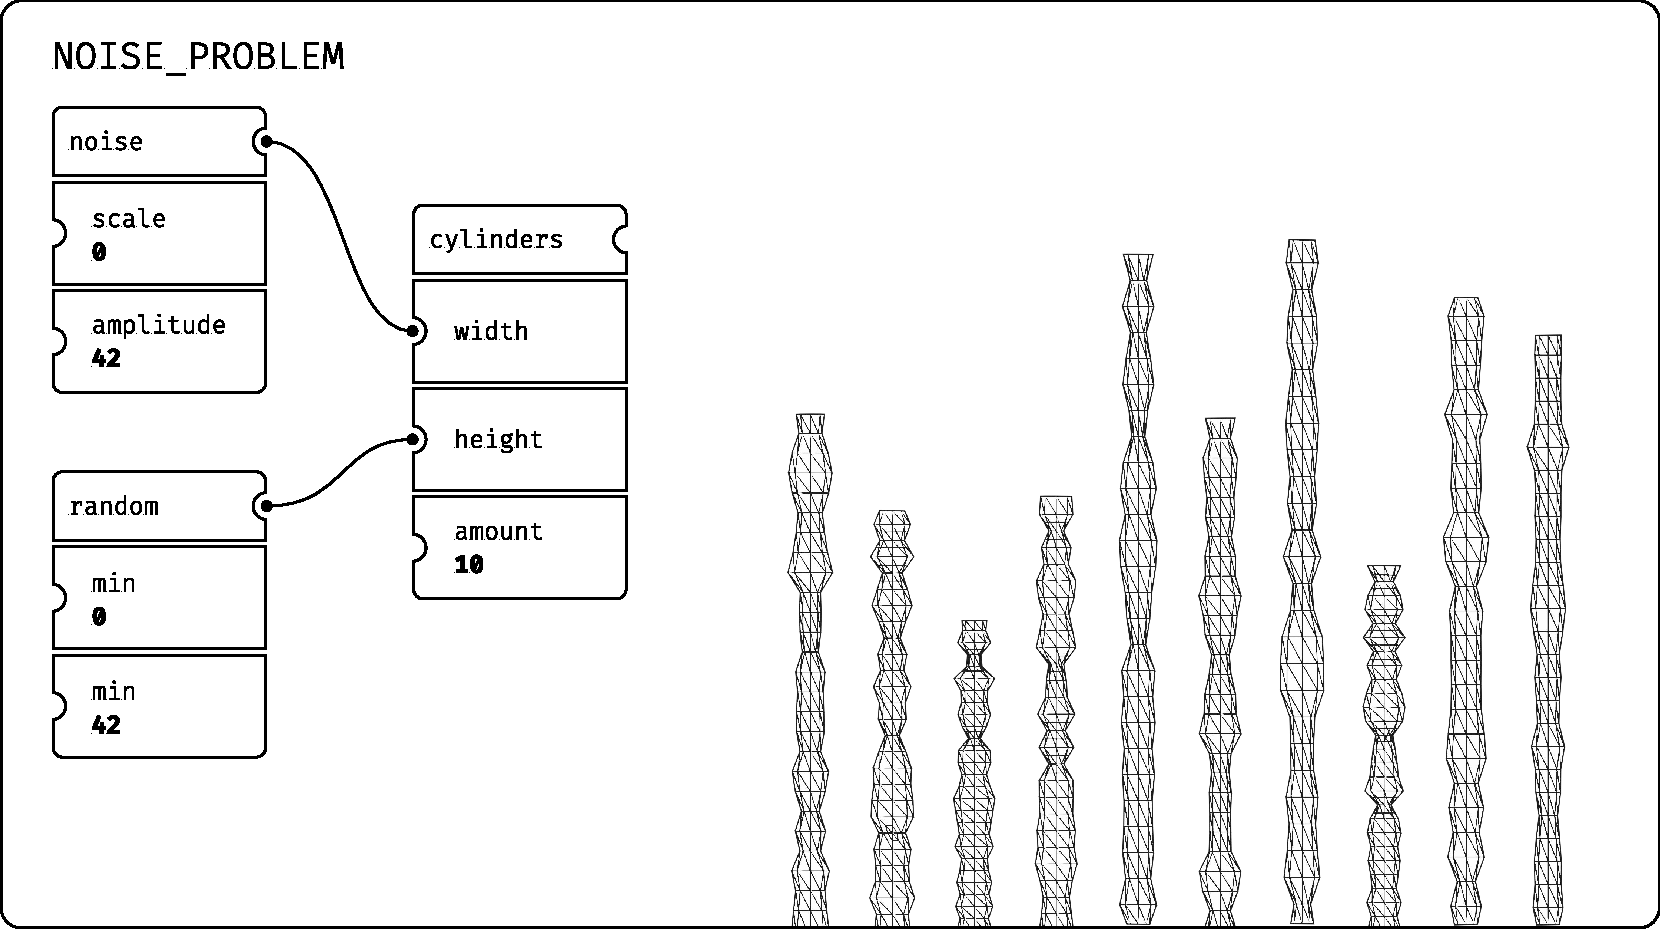
\includegraphics[width=0.8\textwidth]{./graphics/NOISE_PROBLEM.pdf}
  \caption{Problemdarstellung}
  \label{fig:noise_problem}
\end{figure}

\subsubsection*{Lösung}

Eine Lösung für dieses Problem ist die Einführung von parametrisierten Nodes. Das heißt bestimmte Nodes geben kein Ergebnis zurück, sondern eine parametrisierte Version ihrer selbst, die dann von anderen Nodes evaluiert werden kann.
\br
Dies hat den entscheidenden Vorteil das andere Nodes frei entscheiden können, wo und wie oft sie ihre Argumente evaluieren.
Außerdem kann dies implementiert, ohne die Runtime zu beeinflussen, da die Ausführung der Nodes weiterhin in einer Richtung verläuft.
\br
Die \topic{cylinder} Node im vorherigen Beispiel könnte zum Beispiel bei der Evaluierung der \topic{random} Node ein \topic{seed} übergeben.
\br
Eine Herausforderung in der Implementierung dieser Lösung besteht darin das jedes Argument nun entweder ein direkter Wert, der von den Nutzern über das \link[node_interface]{Node-Interface} festgelegt wird, oder ein Teil das gesamten \link[node_graph]{Node-Graphen} sein kann.
\br
Da der \link[runtime_executor]{Runtime-Executor} aus Gründen der Erweiterbarkeit möglichst wenig spezifische Informationen über einzelne Nodes brauchen soll,
habe ich mich dazu entschieden das die einzelnen Nodes sich selber serialisieren und diese Serialisierung als Ergebnis zurückgeben.
\br
Die erste Implementierung bestand darin das die Nodes ein serialisiertes JSON-Objekt zurückgeben. Dies hatte den Vorteil, dass einzelne Argumente zu Debugging-Zwecken menschenlesbar und die Serialisierung relativ einfach war. Die Performance war jedoch nicht optimal, da die Serialisierung und Deserialisierung relativ aufwendig ist. Des Weiteren hatte jede Node jetzt eine Abhängigkeit zu \href{ https://serde.rs/ }{Serde} (Der Standardbibliothek für Serialisierung in Rust), was die Dateigröße der WebAssembly-Module deutlich vergrößerte.
\br
Die aktuelle Version benutzt eine eigene Binär-Serialisierung. Diese ist schneller und die Dateigröße der WebAssembly-Module ist kleiner. Der Nachteil ist das die Serialisierung nicht mehr menschenlesbar und die Implementierung komplexer ist. 
\\
Die Grundidee ist es Nodes als ein Array aus 32Bit Integer darzustellen, die erste Stelle des Arrays enkodiert den Typ der Node, die darauffolgenden Stellen sind die Argumente. Die einzelnen Argumente sind entweder eine Zahl oder die enkodierte Version einer anderen Node.
Gleitzahlen sind 32 Bit nach dem IEEE-754 Standard und können dank der gleichen Größe ohne weiter Anpassungen im Array gespeichert werden. 
\br
Da WebAssembly, sowie auch Rust keine verschachtelten Arrays unterstützen, muss dieser Array in einen linearen Array umgewandelt werden. 
Der \qt{Recursive-Length Prefix Serialization} Algorithmus von Ethereum war ein guter Ansatz, ist jedoch nicht für die Anforderungen dieser Anwendung optimiert, da er für Strings ausgelegt ist. 
\cite{wood2024ethereum}
\br
Das aktuelle Binärformat besteht darin jede Klammer in einem verschachtelten Array durch zwei 32 Bit Integer zu enkodieren. 
Die erste Stelle gibt, an ob es sich um eine öffnende oder schließende Klammer handelt, die zweite Stelle gibt den Abstand zur nächsten Klammer an.

\begin{figure}[htbp]
  \centering
  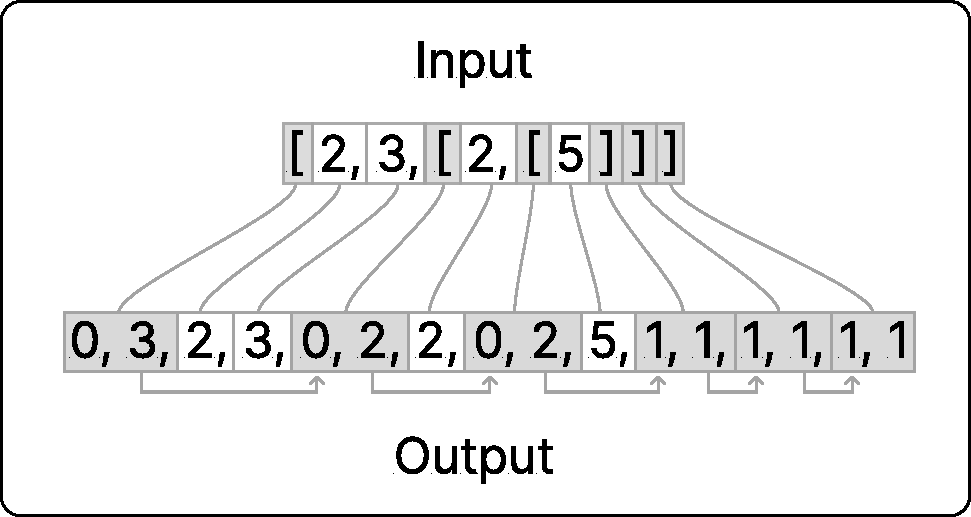
\includegraphics[width=0.8\textwidth]{./graphics/ENCODING_SCHEME.pdf}
  \caption{Visualisierung der Binär-Serialisierung}
  \label{fig:encoding_scheme}
\end{figure}

Eine Limitierung dieser Implementierung ist das 32 Bit integer nur Zahlen bis maximal $2^{31}-1$ darstellen können. Dies beschränkt die Länge eines Arrays auf $2,147,483,647$ Elemente. Für diese Anwendung ist das jedoch mehr als ausreichend.

\subsubsection*{O-Notation}
Die O-Notation der \link[code_nested_encoding]{Beispiel-Implementierung} ist $O(n)$, wobei $n$ die Anzahl der Elemente in der Serialisierung ist. Tatsächlich können wir aber während der Laufzeit oft einen einfacheren Algorithmus benutzen, da die meisten parametrisierten Nodes nicht tief in die Verschachtelung gehen, sondern nur die obersten Elemente extrahieren und nachher wieder zusammenfügen. 
\br
Beispielsweise nimmt eine \topic{math} Node, ihre Operation (addieren, subtrahieren...) und zwei Zahlen entgegen und fügt diesen Argumenten nur einen Integer zur Identifizierung hinzu. Dafür können wir Algorithmen benutzen der nur die obersten Elemente \link[code_nested_splitting]{extrahieren} und wieder \link[code_nested_joining]{zusammenfügen}.  Diese Algorithmen haben eine O-Notation von $O(1)$.


\subsection{Design}

Die Anwendung wurde so designt, dass sie möglichst einfach und intuitiv zu bedienen ist. Dafür wurde ein sehr simples zweispaltiges Layout gewählt. Auf der rechten Seite befindet sich das \link[node_interface]{Node-Interface} und auf der linken Seite die 3D-Visualisierung der entstandenen Pflanze. Zudem gibt es auf der rechten Seite eine Symbolleiste die den Zugriff auf verschiedene Untermenüs erlaubt. Diese sind aber standardmäßig ausgeblendet, um die Übersicht zu erhöhen.

\begin{figure}[hbtp]
  \centering
  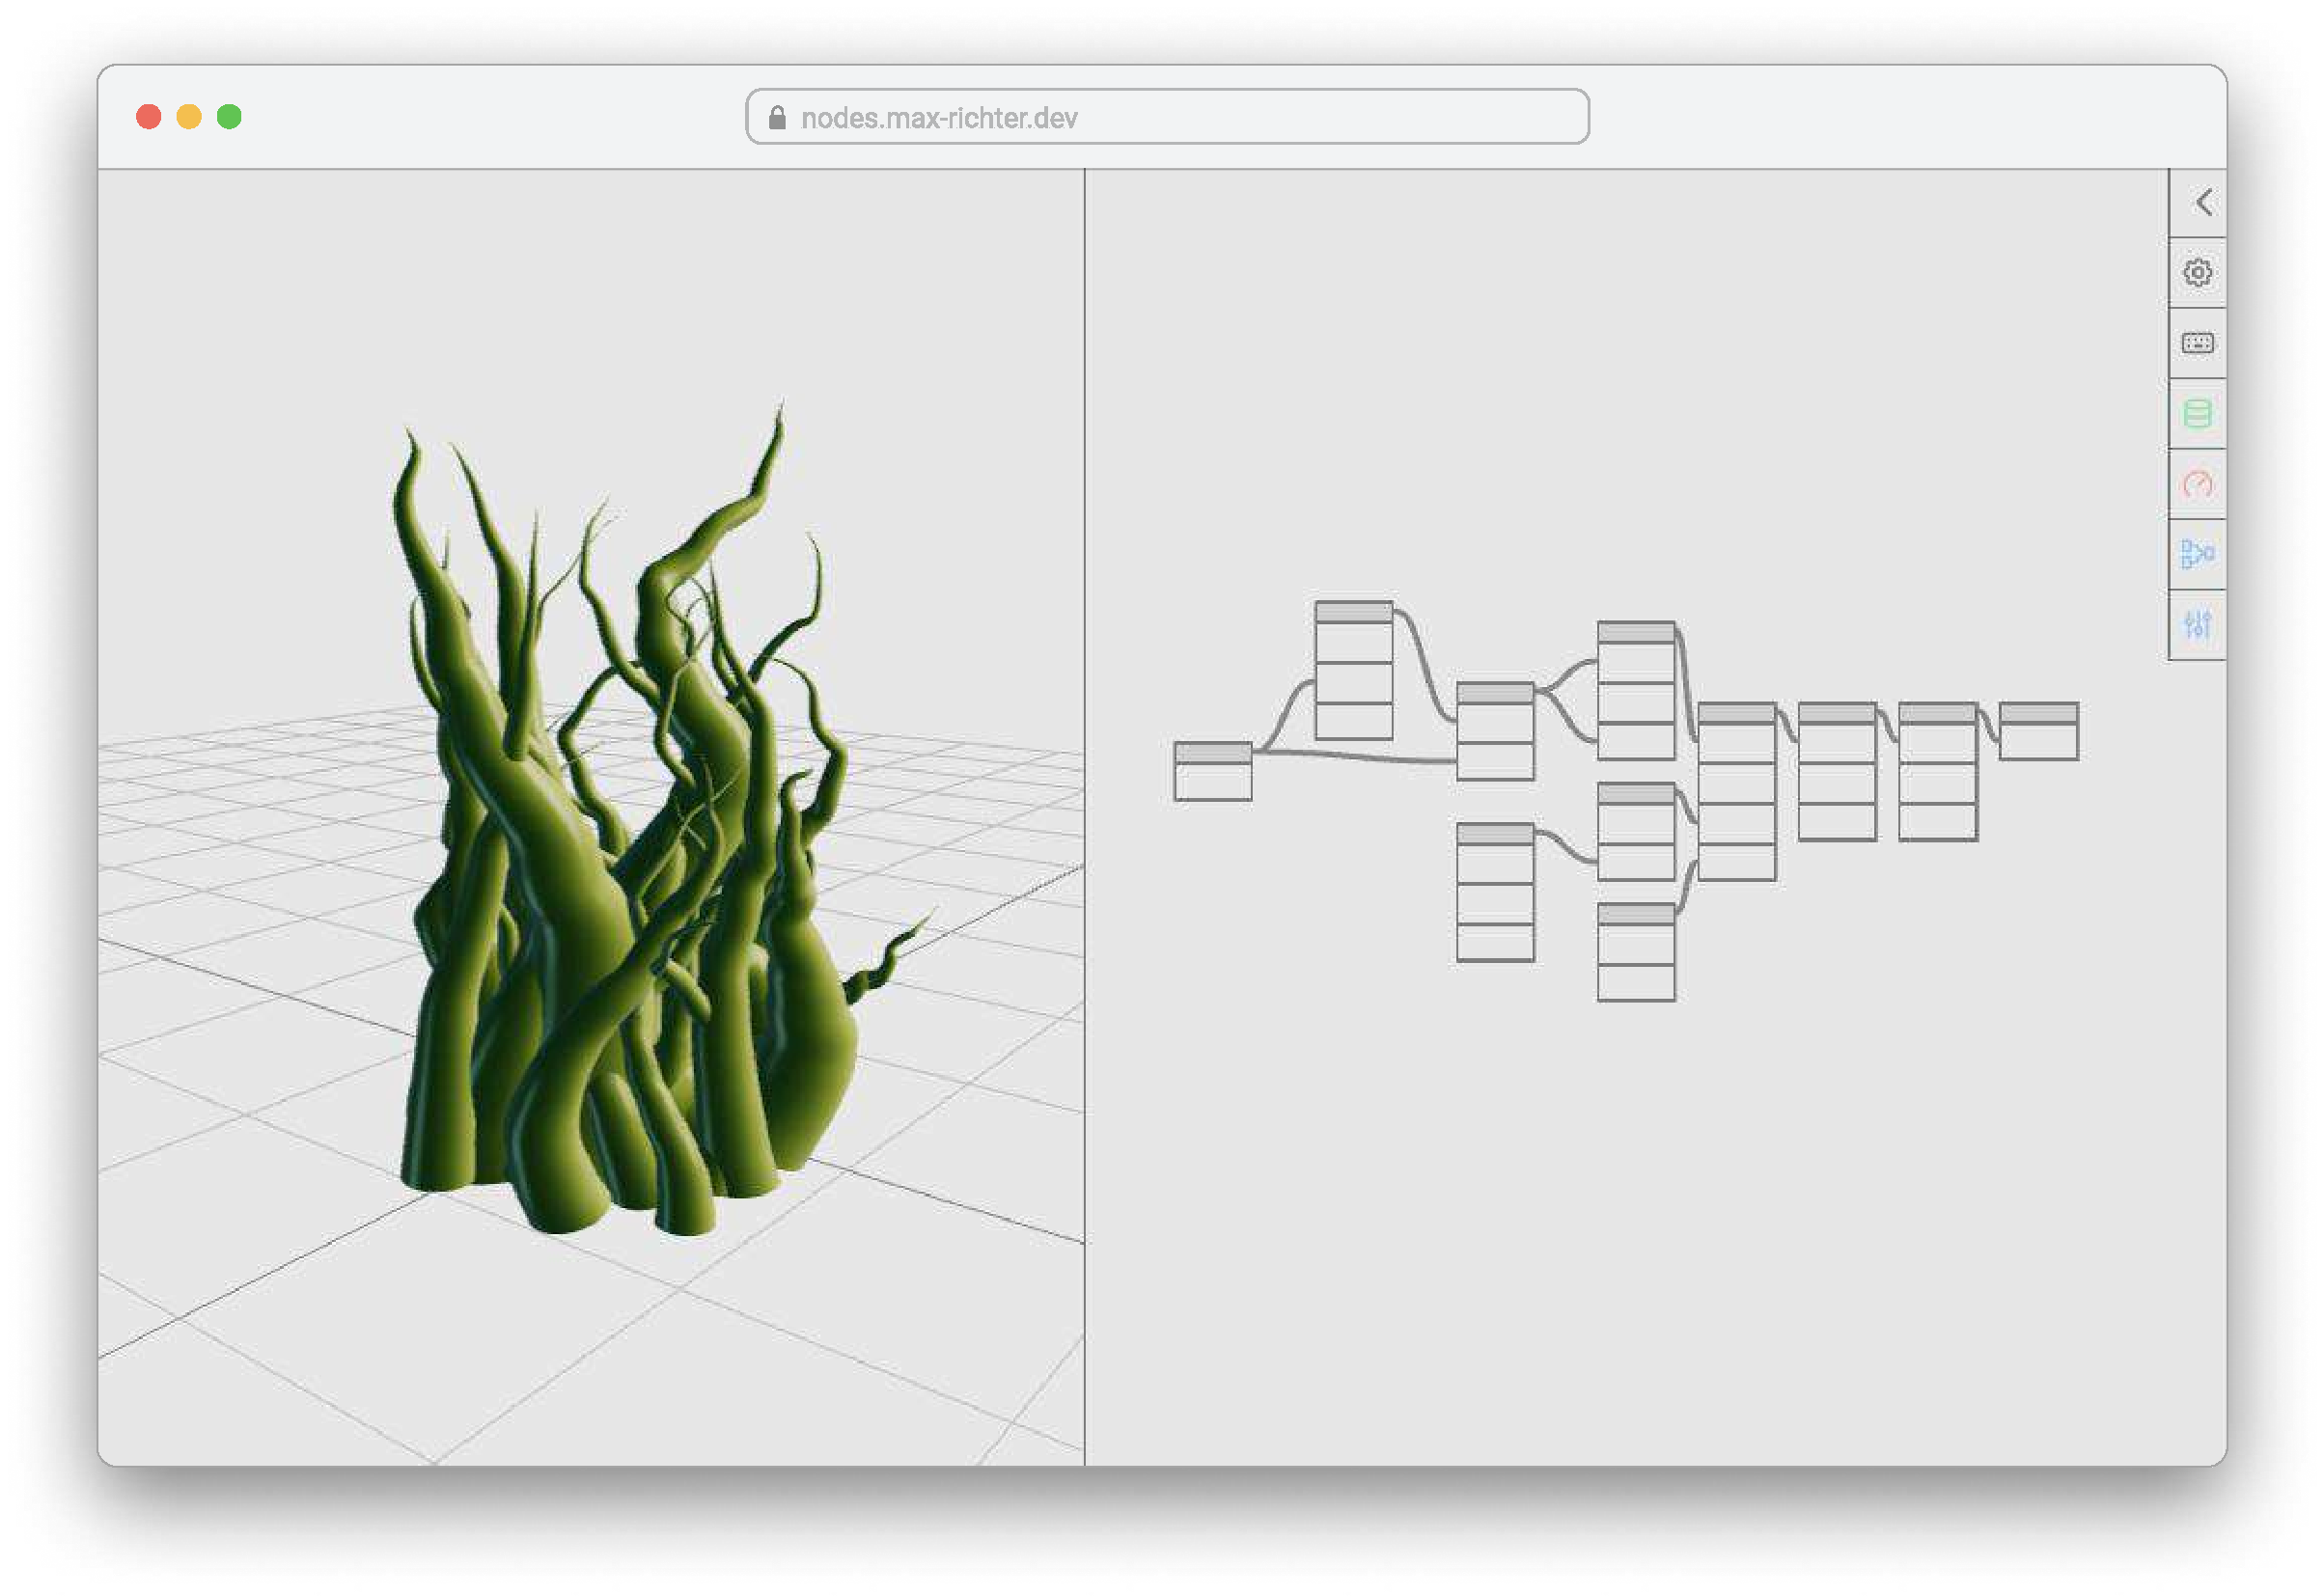
\includegraphics[width=1\textwidth]{graphics/layout_light.pdf}
  \caption{Screenshot der Anwendung im Light-Mode}
  \label{fig:screenshot_nodarium}
\end{figure}

\pagebreak

\subsubsection{Farbgebung}

Da es sich bei der Anwendung um ein Tool für die Entwicklung von 3D-Modellen handelt, wurde eine Farbgebung die möglichst unaufdringlich und minimalistisch ist.
Zur Entwicklung der Farbpalette wurde ein neutrales dunkles Grau gewählt von dem aus den zwei Dunklere und drei hellere Farben abgeleitet wurden. Aus diesen 6 Farbtönen wurden dann die einzeln Farbschemas für die Anwendung abgeleitet. Außerdem wurde ein High-Contrast-Mode implementiert, der die Farben so anpasst, dass sie auch für Nutzer/innen mit Sehschwäche gut erkennbar sind.

\subsubsection{Node Design}


\begingroup
\setlength\intextsep{4pt}
\begin{minipage}{\linewidth}
\begin{wrapfigure}{L}{0.48\textwidth}
    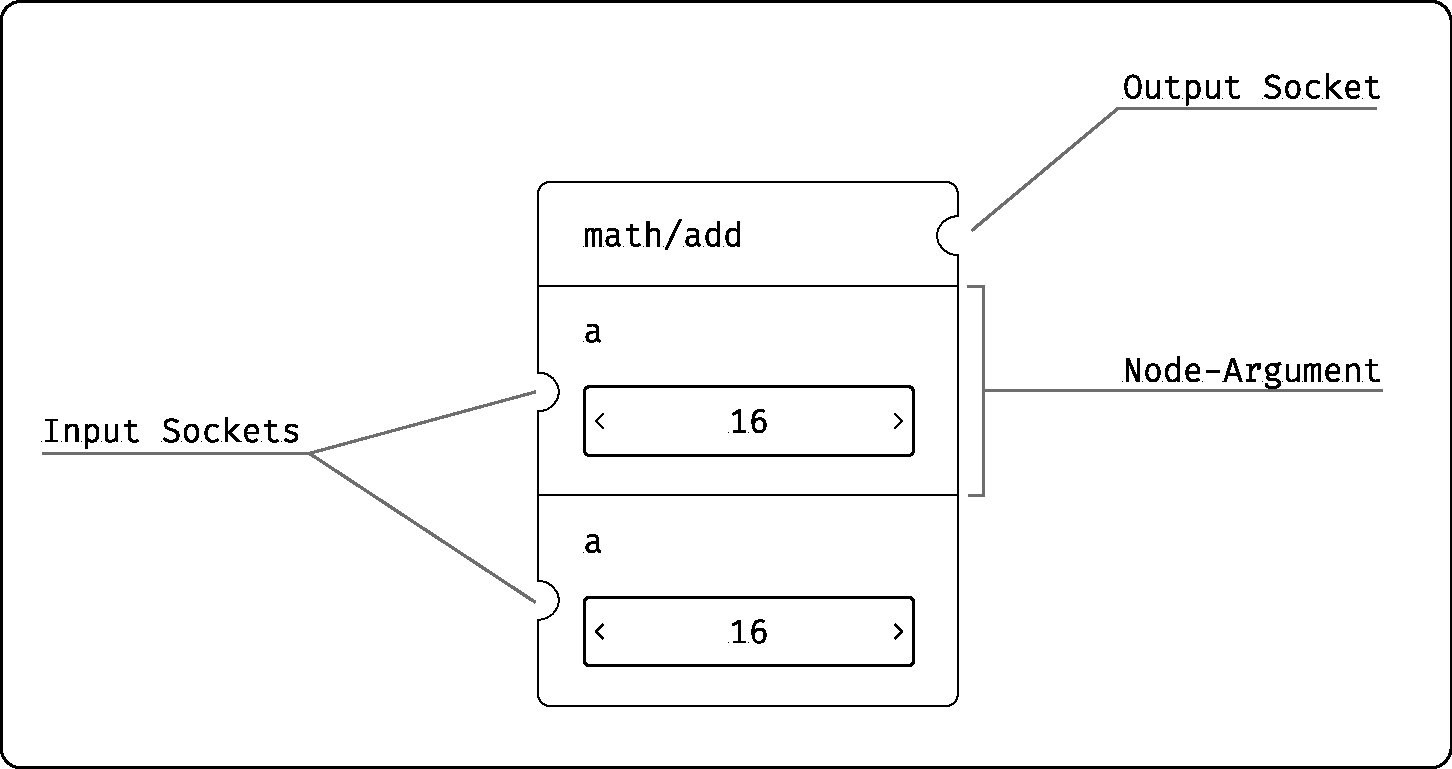
\includegraphics[width=0.47\textwidth]{graphics/NODE_ANATOMY.pdf}
    \caption{Anatomie einer Node}
    \label{sec:NODE_ANATOMY}
\end{wrapfigure}

Das Design der einzelnen Nodes ist stark an Blenders Design angelehnt. Die Struktur einer Node ist in Abbildung \ref{sec:NODE_ANATOMY} dargestellt. 

Ein großer limitierender Faktor beim Design der Nodes ist der vertikale Raum den eine Node einnimmt. Da bei der Entwicklung einer Node die Anzahl der Argumente schnell anwachsen kann, kann auch die vertikale Größe schnell anwachsen. 
Um dieses Problem zu beheben habe ich den \link[node_input]{Node-Inputs} eine Einstellung hinzugefügt, die diesen Input in ein Untermenü auf der rechten Seite versteckt. 
\end{minipage}
\br
\endgroup

\begin{figure}[htpb]
  \centering
  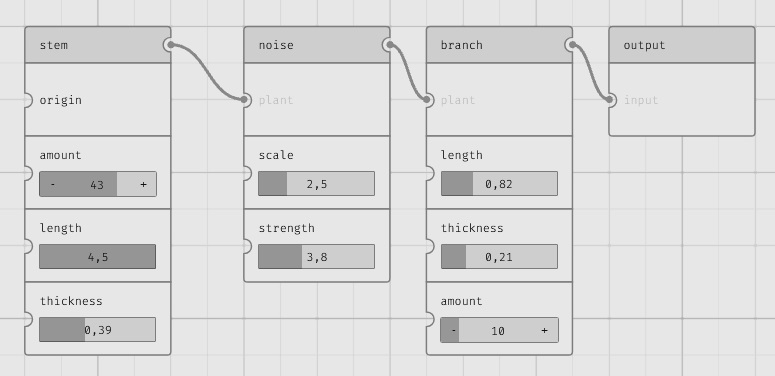
\includegraphics[width=1\textwidth]{graphics/node_graph.jpg}
  \caption{Screenshot eines \link[node_graph]{Node-Graphen}}
  \label{fig:node_graph_screenshot}
\end{figure}


\section{Implementierung}
Die Anwendung wurde in einem Mono-Repository entwickelt, das die einzelnen Komponenten als eigenständige Pakete enthält. Dies hat den Vorteil das alle Komponenten gemeinsam entwickelt, versioniert und getestet werden können. 
\br
Außerdem unterstützen die beiden Paket-Manager \href{https://pnpm.io/}{pnpm} und \href{https://crates.io/}{cargo} das Arbeiten mit 
Mono-Repositories sehr gut. 

\subsection{Nodes}
\cmt{Validierung der node-definition durch rust macro und zod}

\subsection{Runtime-Executor}
\cmt{allgorithmus - recursive preprocessing}

\subsection{Node-Interface}
Der Fokus bei der Implementierung lag darauf das Interface so simpel und performant wie möglich zu gestalten. Hierfür wurde eine hybride Darstellung aus HTML und WebGL Elementen entwickelt. HTML Elemente bieten hierbei den Vorteil, das sie einfach zu gestalten sind und gute Interaktionsmöglichkeiten bieten. Bei einer großen Anzahl sich bewegender HTML Elemente sinkt jedoch die Performance. 
Deswegen wird ab einer bestimmten Zoom-Stufe die Darstellung der Nodes in ein WebGL Canvas gerendert. Dies hat den Vorteil, dass die Performance bei einer großen Anzahl von Nodes konstant bleibt. 
Zur weiteren Verbesserung der Performance werden die abgerundeten Ecken und Rahmen der einzelnen Nodes per \href{https://en.wikipedia.org/wiki/Signed_distance_function}{Signed Distance Function} gerendert.

\pagebreak


\section{Evaluation}


\subsection{Anforderungen}


\subsubsection{Performance}

Die Performance wurde anhand drei Benchmarks auf drei Geräten jeweils in Chrome (v124) und Firefox (v125). Die drei Benchmarks waren:

\begin{itemize}
  \item test\_a: 6 Nodes generieren 2,1 Millionen Polygone
  \item test\_b: 228 Nodes generieren 127 Tsd. Polygone
  \item test\_c: 228 Nodes generieren 1 Million Polygone
\end{itemize}

Die einzelnen Benchmarks wurden End-to-End gemessen, das heißt die Zeit die benötigt wird, um den \link[node_graph]{Node-Graphen} auszuführen, die Polygone in der Szene anzuzeigen und die Szene zu rendern.
\br
Die drei Geräte waren ein Smartphone (Google Pixel 4a 2020, 8GB RAM, Snapdragon 730G), ein Laptop (Razer Blade Stealth 2016, 16GB RAM, i7-7500U) und eine Workstation (Intel I7-6700K, 16GB RAM, Nvidia GTX1060). Dargestellt wird die Durchschnittsdauer von 500 Durchläufen und die Standardabweichung.

\begin{table}[htbp]
\begin{tabular}{|l|l|l|l|}
\hline
Firefox      & Smartphone                 & Laptop                 & Workstation                 \\ \hline
test\_a      & 208.34ms \stdev{31.51}     & 111ms \stdev{20.76}    & 105.75ms \stdev{12.33}      \\ \hline
test\_b      & 42.07ms \stdev{11.24}      & 22.66ms \stdev{5.63}   & 20.12ms \stdev{3.79}        \\ \hline
test\_c      & 168.66ms \stdev{54.74}     & 67.58ms \stdev{40.03}  & 65.33ms \stdev{13.63}       \\ \hline
\end{tabular}
\end{table}


\begin{table}[htbp]
\begin{tabular}{|l|l|l|l|}
\hline
Chrome           & Smartphone                & Laptop                & Workstation                \\ \hline
test\_a          & 347.02ms  \stdev{30.6}    & 127.97ms \stdev{7.28} & 136.92ms \stdev{3.28}      \\ \hline
test\_b          & 77.19ms \stdev{31.75}     & 21.1ms  \stdev{6.01}  & 18.12ms \stdev{3.74}       \\ \hline
test\_c          & 316.73ms \stdev{62.54}    & 65.46ms \stdev{15.65} & 67.62ms \stdev{23.03}      \\ \hline
\end{tabular}
\end{table}

\subsubsection{Erweiterbarkeit}
\cmt{Neue Nodes können einfach hinzugefügt werden}
\cmt{Macros + Dokumentation}

\subsubsection{Usability}
\cmt{Intuitiv}
\cmt{Viele Tastaturkürzel}
\cmt{Drag and Drop}

\subsection{Forschungsfragen}

\section{Fazit}
\cmt{Joah, schnieke würd ich mal sagen}

\cmt{WASM eignet sich gut}

\cmt{WASM -> low level -> schnell}

\cmt{WASM -> low level -> komplex}

\cmt{WASM -> single file exec}

\cmt{Lose Kopplung -> flexibel}

\section{Ausblick}
\cmt{Remote Hosting für Nodes}

\cmt{WebAssembly Component Model -> More speed?}

\cmt{Implementierung der Namespaces}

\cmt{Integration der Runtime in Plugins}

\cmt{Mehr Nodes für Pflanzen}

\cmt{Entwicklung einer visuellen Identität}

\cmt{Erweitern der Dokumentation}

\pagebreak
\section{Glossar}

\subsection{Node}
\label{sec:node}
Einzelner Baustein eines \hyperref[sec:node_graph]{Node-Graphs}. Eine Node funktioniert etwa wie eine Funktion in einer textuellen Programmiersprache. Sie nimmt \hyperref[sec:node_argumente]{Node-Argumente} entgegen, verarbeitet diese und gibt ein Ergebnis zurück. 


\subsection{Node-Definition}
\label{sec:node_definition}
Eine Node ist quasi eine Instanz einer Node-Definition. Eine Node-Definition definiert die Struktur einer Node. Sie enthält Informationen über die Inputs und Outputs einer Node und die Funktion, die die Node ausführt.

\subsection{Node-Graph}
\label{sec:node_graph}
Node-Graphs sind ein gerichteter \link[PURE_GRAPH]{azyklischer Graph (DAG)} von \link[node]{Nodes}. Sie bestehen aus einer Menge von Nodes und deren Verknüpfungen. 

\subsection{Node-Argumente}
\label{sec:node_argumente}
Node-Argumente sind die Eingabeparameter einer Node. Ein Node-Argument kann entweder direkt über das Interface in einer \link[node]{Node} definiert werden oder indem der User einen Output-Socket einer anderen Node mit dem \link[node_socket]{Node-Socket} eines Node-Argument verknüpft.

\subsection{Node-Socket}
\label{sec:node_socket}
Node-Sockets sind die Verbindungspunkte zwischen \link[node]{Nodes}. Eine Node hat mehrere Input-Sockets und einen Output Socket.

\pagebreak

\section{Beispiel-Code}
\subsection{Binär-Serialisierung}
\label{sec:code_nested_encoding}

\begin{figure}[htbp]
  \begin{code}
    \begin{minted}{typescript}
// Recursiver Datenstruktur für verschachtelte Arrays
type SparseArray = (number | number[] | SparseArray<T>)[];

// Kodiert ein verschachteltes Array
export function encodeNestedArray(array: SparseArray): number[] {
  const encoded = [0, 0]; // Initialisiere das Ergebnis
  let missingBracketIndex = 1; // Abstand zur letzten Klammer

  for (let index = 0; index < array.length; index++) {
    const item = array[index];
    if (Array.isArray(item)) {
      // Aktualisiere die letzte Klammer
      encoded[missingBracketIndex] = encoded.length - missingBracketIndex;
      if (item.length === 0) {
        // Behandle leere Arrays
        encoded.push(0, 1, 1, 1);
      } else {
        // Kodiere rekursiv nicht-leere Arrays
        const child = encodeNestedArray(item);
        encoded.push(...child);
      }
      // Aktualisiere den Abstand für die zuletzt geöffnete Klammer
      missingBracketIndex = encoded.length - 1;
    } else {
      // Behandle Nicht-Array-Elemente
      encoded.push(item);
      // Aktualisiere den Abstand für die zuletzt geöffnete Klammer
      if (missingBracketIndex) encoded[missingBracketIndex] = index + 2;
    }
  }

  return [...encoded, 1, 1];
};
    \end{minted}
  \end{code}

  \caption{Beispiel-Code Binär-Serialisierung (TypeScript)}
  \label{sec:data_nested_encoding}

\end{figure}

\pagebreak

\subsection{Binär-Splitting}
\label{sec:code_nested_splitting}

\begin{figure}[htbp]
  \begin{code}
    \begin{minted}{rust}
pub fn split_args(args: &[i32]) -> Vec<&[i32]> {
    let mut out_args: Vec<&[i32]> = Vec::new();
    let mut depth = 0;
    let mut i = 0;
    let mut start_index = 0;
    let mut next_bracket_index = 0;
    let len = args.len();

    while i < len {
        // Wenn wir uns an einer Klammer befinden
        if i == next_bracket_index {
            next_bracket_index = i + args[i + 1] as usize + 1;
            // Wenn die Klammer öffnet
            if args[i] == 0 {
                if depth == 1 {
                    start_index = i;
                }
                depth += 1;
            } else {
                depth -= 1;
                if depth == 1 {
                    out_args.push(&args[start_index..i + 2]);
                    start_index = i + 2;
                }
            }
            i += 2;
            continue;
        } else if depth == 1 {
            out_args.push(&args[i..i + 1]);
            start_index = i + 1;
        }
        i += 1;
    }

    out_args
}
    \end{minted}
  \end{code}

  \caption{Beispiel-Code Binär-Splitting (Rust)}

\end{figure}

\pagebreak

\subsection{Binär-Joining}
\label{sec:code_nested_joining}
\begin{figure}[htbp]
  \begin{code}
    \begin{minted}{rust}
pub fn concat_args(data: Vec<&[i32]>) -> Vec<i32> {
    // 4 um die erste/letzte Klammer zu berücksichtigen
    let mut total_length = 4; 

    for vec in &data { // Berechnen der Gesamtlänge, um Neuzuweisungen zu vermeiden
        if vec.len() == 1 {
            total_length += 1;
        } else {
            total_length += vec.len(); // +4 für die Klammern um jeden Subarray
        }
    }

    let mut result = Vec::with_capacity(total_length);

    result.push(0); // Öffnende Klammer
    result.push(1);

    let mut last_closing_bracket = 1;

    for vec in data.iter() {
        if vec.len() == 1 {
            result.push(vec[0]);
            result[last_closing_bracket] += 1;
            continue;
        } else {
            result.extend_from_slice(vec);
            last_closing_bracket = result.len() - 1;
            result[last_closing_bracket] = 1;
        }
    }

    result.push(1); // Schließende Klammer
    result.push(1);

    result
}

    \end{minted}
  \end{code}

  \caption{Beispiel-Code Binär-Joining (Rust)}

\end{figure}

\pagebreak
\section{Literaturverzeichnis}

\printbibliography

\end{document}
